%\documentclass[a4paper]{article}
%\documentclass[review]{elsarticle}
\documentclass[]{elsarticle}

%% Language and font encodings
\usepackage[english]{babel}
\usepackage[utf8x]{inputenc}
\usepackage[T1]{fontenc}

%% Sets page size and margins
\usepackage[a4paper,top=3cm,bottom=2cm,left=3cm,right=3cm,marginparwidth=1.75cm]{geometry}

%% Useful packages
%\usepackage{amsmath}
%\usepackage{graphicx}
%\usepackage{mathcomp}

\usepackage[colorinlistoftodos, textsize=small]{todonotes}
\usepackage[colorlinks=true, allcolors=blue]{hyperref}
\usepackage{lineno,hyperref}
\newcommand\rewrite[1]{\todo{rewrite #1}}
\newcommand\extend[0]{\todo{extend}}
\newcommand\lavrov[1]{\todo[inline]{Lavrov: #1}}

\title{Mammalian CPG neuro-simulation results}

\begin{document}

\begin{frontmatter}

\author[inst1]{Max Talanov 1}
\ead{max.talanov@gmail.com}
\author[inst1]{Alina Suleimanova}
\ead{sulemanovaaa@icloud.com}
\author[inst1]{Alexey Leukhin}
\ead{alexey.panzer@gmail.com}
\author[inst1]{Fail' Gafarov}
\ead{fgafarov1977@gmail.com}
\author[inst2]{Carlos A. Cuellar}
\ead{Carlos.A.Cuellar@mayoclinic.org}
\author[inst2]{Riazul Islam}
\ead{Riazul.Islam@mayoclinic.org}
\author[inst1,inst2,inst3,inst4,*]{Igor Lavrov}
\ead{Igor.Lavrov@mayoclinic.org}

\address[inst1]{Kazan Federal University, Kazan Russia.}
\address[inst2]{Department of Neurologic Surgery, Mayo Clinic, Rochester, MN, USA.}
\address[inst3]{Department of Physiology and Biomedical Engineering, Mayo Clinic, Rochester, MN, USA}
\address[inst4]{Department of Neurology, Mayo Clinic, Rochester, MN, USA}
\address[*]{Corresponding author}

\begin{abstract}

\ldots

\end{abstract}

\begin{keyword}
CPG \sep computational simulation \sep spinal cord injury \sep spinal cord stimulation \sep spinal cord motor-evoked responses \sep neuro-simulation
\end{keyword}
\end{frontmatter}

%\linenumbers

\section{Introduction}

The modeling of biological neural circuits is an important direction in development  of artificial neural network \cite{bekka2002use}. \todo{actually this is wrong} 
At the same time, computer simulations of neuronal circuits require information regarding physiological and anatomical organization of the nervous system, which is not accessible by direct measurements \cite{prentice2001artificial}. Precise values of many basic parameters of neurons and networks, as well as neuronal interactions are usually not available and commonly substituted by theoretical models (Soares and Cortez, 1999; Cruz, et al., 2000)\todo{Igor we still need this articles} \cite{bizzi1991computations} and in fact all currently available computer simulations of biological circuits are developed with great level of approximation. Important applications of biological circuitry modeling primary related to development of motor and sensorial neuroprosthesis, including the simulation of biological circuits with increasing degrees of complexity and automation \cite{donaldson1997neuroprostheses,lauer1999eeg}. 

Previously we successfully implemented spinal cord stimulation techniques to identify components of spinal cord circuitry involved in recovery of stepping in complete spinal rats and we found that electrical epidural stimulation (EES) can induce four types of motor evoked electrical responses in the hind limb muscles \cite{gerasimenko2006spinal,lavrov_plasticity_2006}.

Observed correlation between restoration of spinal cord polysynaptic responses after spinal cord injury (SCI) and recovery of stepping facilitated with epidural stimulation \cite{lavrov2008,lavrov_plasticity_2006} suggests on possibility for the identification of specific parts of spinal circuitry and mechanisms involved in the spinal cord plasticity after injury. Accounting the complicity of changes in the spinal cord and in synaptic organization after injury, we proposed a novel model, which systematizes our previous experimental findings and provides insight on functional organization of spinal locomotor networks. Comparing \emph{in vivo} and \emph{in silico} results we investigated the effect of (1) modulation in sensory input (modulation of parameters of EES, i.e. frequency, amplitude, and geometry of stimulation; modulation of sensory input from treadmill, i.e. speed, direction, and load; surgical elimination of sensory input, etc), (2) electrical and pharmacological modulation of the spinal circuitry (spinal networks reorganization at different time after injury, modulation of synaptic activity with pharmacological pretreatment with strychnine and quipazine), and (3) modulation in supraspinal input (comparison between control, anesthetized animals, spinal cord injured animals).

\section{Methods} 

Data for this study were collected during previously published works (2006--2018) on Sprague Dawley rats, 270--300 g body weight and evaluated in regards of circuitry organization and modulation of spinal cord motor evoked potentials. The experimental procedures in these studies comply with the guidelines of National Institute of Health Guide for the Care and Use of Laboratory Animals. Surgical procedures, injury model, implantation techniques, stimulation and recording procedures, and animal care was described elsewhere \cite{roy1991emg,talmadge2002mechanical,ichiyama2005hindlimb,lavrov_plasticity_2006,lavrov2008}.

\subsection{Data collection and analysis} 

All recordings were collected at stimulation intensities between 0.5 V to 10 V. Comparisons of the responses at different voltages were used to identify the onset and amplitude of the early response (ER), medium response (MR), late response (LR), and polysynaptic components (PC). These three responses were modulated during each test session, and were clearly voltage-dependent. All electrophysiological recordings from the muscles were analyzed within a 27 ms period after the stimulus artifact and were divided into four windows based on the onset latencies of the four types of responses, i.e., 1.5 to 6.5 ms for the ER, 6.5 to 10.5 ms for the MR, 10.5 to 13.5 ms for the LR, and 13.5 to 27 ms for the PC. The maximum peak-to-peak amplitude for each response was calculated as an average of 10 responses and reported as a percentage of the control value. Modulation of mono- and polysynaptic components were assessed in vivo freely moving rats and in silico on designed hypothetical spinal circuitry model (see below Section \ref{sec:cir}). Motor activity from in vivo animals was induced by a combinations of sensory input, supraspinal input, and the state of the spinal circuitry, and was correlated with the input and output of computer model, to evaluate proposed organization of spinal circuitry.

\begin{figure}[ht!]
	\centering
	\includegraphics[width=1.0\textwidth]{myogram_FE-Combined.png}
	\caption{
    \todo[inline]{Move the pic to the Figure 3}
    \lavrov{ Fig 3 already has this information}
	The myogram recorded from foot extensor  during stepping facilitated with EES, where 
    MR -- monosynaptic response generated by a reflex arc, 
    LR -- polysynaptic late response generated via CPG.}
	\label{fig:myogram_origin}
\end{figure}

\subsection{Circuitry model} \label{sec:cir}

We propose a novel neuronal model of spinal cord circuitry to explain modulation of MR, LR, and PC components during stepping facilitated with EES or pharmacology and during different functional tests. 
To design the circuitry model we used a ``black box'' approach where hypothetical structure of circuitry was identified based on changes in inputs and outputs. \todo{get rid of second black box}
Changes in inputs, i.e. changes in speed of treadmill, body weight support, changes in supraspinal input, etc, were analyzed in relation to observed output. The structure of hypothetical circuitry was further adjusted based on changes in input-output during modulation of internal circuitry activity, such as reorganization after SCI, changes after adding pharmacological agents. In proposed model, each level from motoneurons to interneurons adds functional flexibility and complexity to the final motor output. Initial circuitry model was design based on our previous observations and consist of multilevel scheme with four main components:

\begin{enumerate}
	\item Monosynaptic level with motoneurons, Ia, Ib interneurons, and Renshaw cells. This level functionally corresponds to the activation of Ia afferent and modulation of monosynaptic reflexes (MR).
	\item Polysynaptic level (or pattern formation) for muscles antagonists involved in movements of ankle joint organized with several mutually inhibited bineuronal modules. This level functionally corresponds to polysynaptic responses (LR and PC).
	\item Initiation level (or pattern generator) that process supraspinal input from MLR (not presented in this model). 
    \todo{I really do not like word eliminated}
	\item Independent components that specify a motion against the gravity processed through the biomechanical structure: bone, tendons, and muscles. These components cannot be completely defined in presented model due to complicity and described as F1 and F2 that pri-F1 and explains the modulation of sensory input and motor output by misbalance, external F2 force, weight bearing features of the limbs, body weight in relation to the gravity. \todo{What is F1 and F2?}
\end{enumerate}

\subsection{Neuron Protocol}

We used updated CPG topology in this simulation in the Neuron simulator \cite{NeuronSimulator}. \rewrite{}
\todo[inline]{add protocols with dynamics}
\begin{description}
	\item Model: Hodgkin–Huxley, Refractory period: 3 ms
	\item Initial membrane potential: $-70$ mV
	\item Inhibitory connection parameters: Model: synapse with STDP
	\item Learning function: Sombrero
	\item Initial weight for $100\%$ inhibition: $-0.08$
	\item EES parameters: Type: NetStim
	\item Interval: 40 Hz (25 ms)
	\item Noise: 0
	\item 1a afferent parameters: Type: SpikeGenerator, Noise: $0.2 (20\%)$
\end{description}

\subsection{NEST Protocol} 

We used updated CPG topology in this simulation in the NEST simulator \cite{Gewaltig:NEST}. \rewrite{}

\begin{description}
	\item Model: $hh\_cond\_exp\_traub$;
	\item Refractory Period: 2 ms \cite{borg1984};
	\item Initial membrane potential $V_m$: $-70.0 mV$; 
	\item Leak reversal potential $E_L: -70.0 mV$; 
	\item Leak conductance: $75.0 ns$;
	\item Time constant of the excitatory synaptic exponential function $tau_syn_ex: 0.2 ms$;
	\item Time constant of the inhibitory synaptic exponential function $tau_syn_in: 3.0 ms$; 
	\item Connection parameters:
	\item Model: $static\_synapse$;
	\item Delay: $1 ms$;
	\item Rule: $fixed\_outdegree; multapses: True; autapses: True$;
\end{description}

\subsection{Statistical analysis}
\todo[inline]{Have to add here analysis for simulation data and comparison between in silico and in vivo results.}

All data reported as means $\pm$ SE. Statistically significant differences were determined using a one-way repeated-measure ANOVA (Student-Newman-Keuls). Values that were not normally distributed were analyzed using the nonparametric Wilcoxon sign-rank test. The statistical significance was set at $p < 0.05$.
\todo[inline]{We have to add here analysis for simulation data and comparison between in silico and in vivo results.}

\section{Results}

\begin{figure}[ht!]
	\centering
	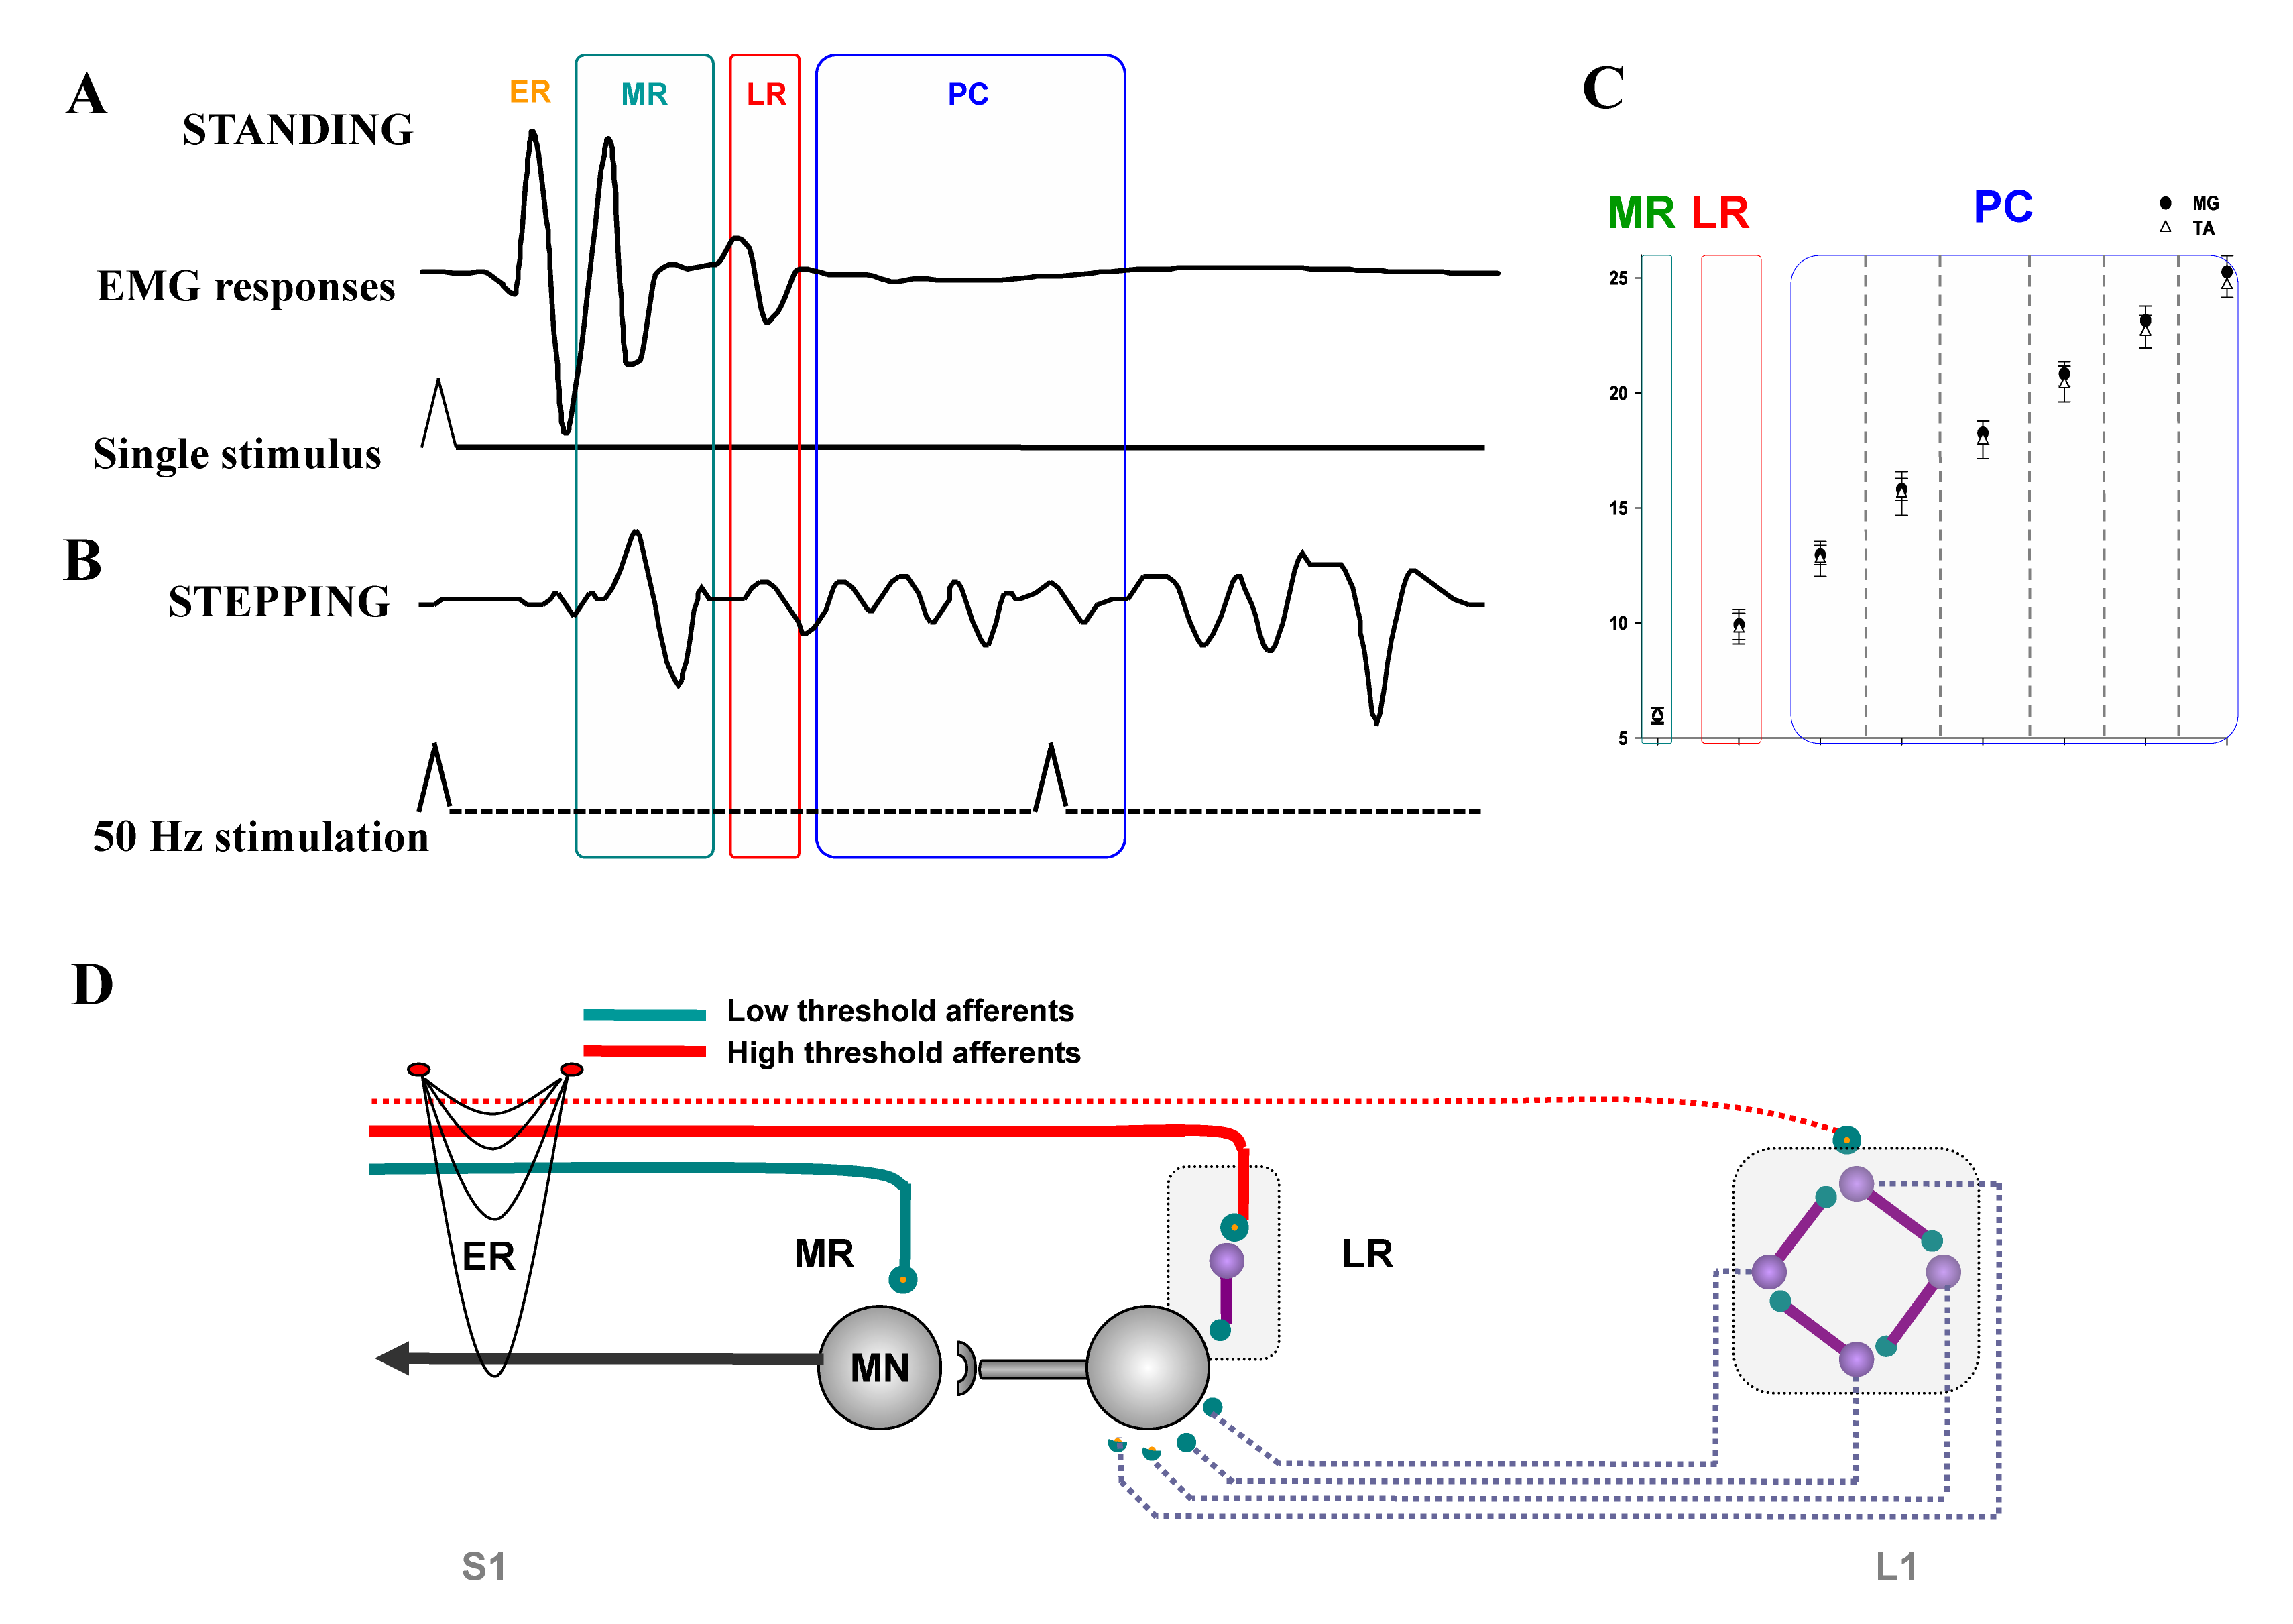
\includegraphics[width=1.0\textwidth]{fig1.png}
	\caption{
    A. Example of spinal cord responses to EES during standing (single shock) and during stepping (50 Hz) at 7 cm/s on a treadmill. 
    B. Latency of MR, LR, and PC responses in the MG and TA muscles during stepping on treadmill. Latencies of spinal cord responses are statistically different (p<0.001) for MG and TA respectively (n=9). 
    C. Numbers of picks (1--6) in PC in A and B correspond to the latency for each pick in PC in C. from \cite{lavrov2008}. 
    D. The schematic organization of simple hypothetic spinal circuitry, representing modulation of MR, LR, and PC with ES.}
    \label{fig:fig1}
\end{figure}

\begin{figure}[ht!]
	\centering
	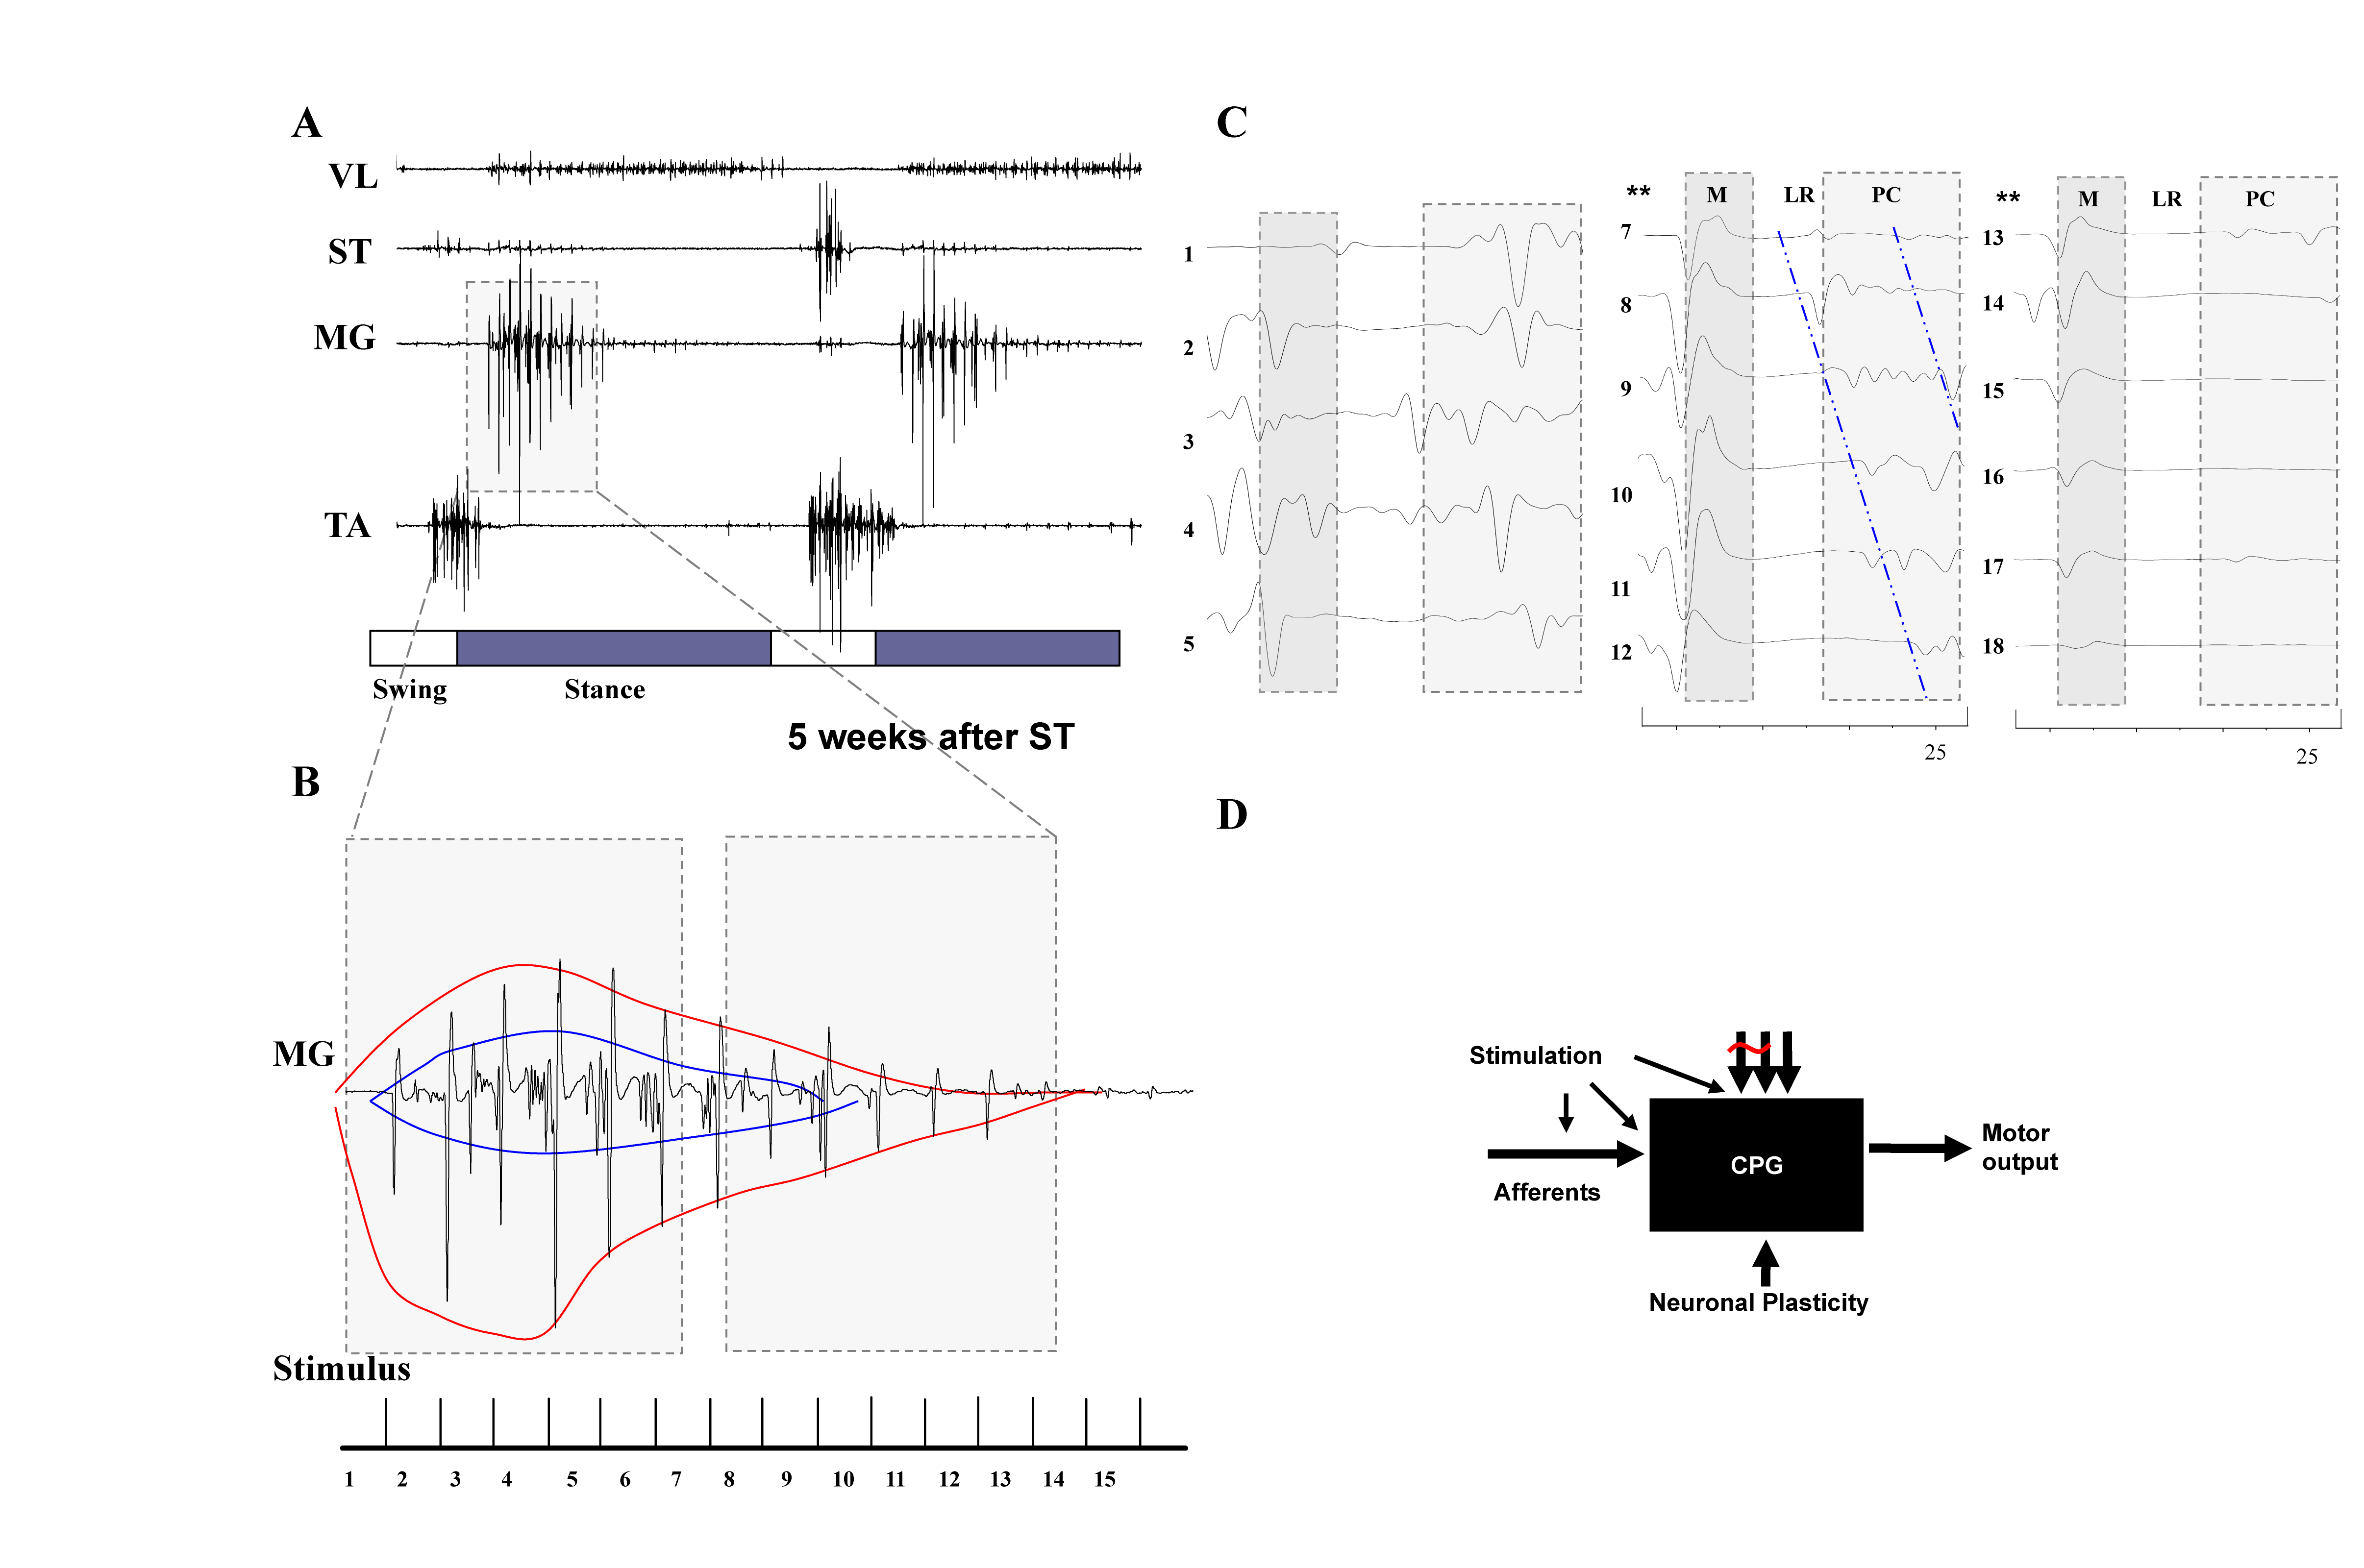
\includegraphics[width=1.0\textwidth]{fig2.png}
	\caption{
    \lavrov{replace C with Fig.1 and remove D}
    A. The formation of EMG bursts in MG and TA muscles from MR, LR and responses of PC during stepping. 
    B. The organization of EMG burst from MR and LR in MG muscle. 
    C. Different modulation of MR and LR in TA and MG muscles,  correspondingly. 
    D. Generated by computer model modulation of monosynaptic responses in flexor and extensor muscles. 
    E. Generated by computer model modulation of polysynaptic activity in extensor muscle. 
    D and E represent different presets of synaptic configurations.}
    \label{fig:fig2}
\end{figure}

\subsection{Spinal cord motor evoked responses induced by ES} 

As we described earlier, spinal cord epidural stimulation produces four types of responses in hindlimb muscles. In standing position, single electrical shock of S1 spinal segment provokes direct early response (ER), monosynaptic middle response (MR) and polysynaptic late response (LR) as described in control \cite{gerasimenko2006spinal} and spinal \cite{lavrov_plasticity_2006} animals (Fig.\ref{fig:fig1}A). The same three responses are observed during rhythmic activity on a moving belt of the treadmill induced by epidural stimulation. In addition to the ER, MR, and LR responses, however, during stepping on a treadmill we observed a polysynaptic complex with a latency > $13.5 ms$ (PC) (Fig.\ref{fig:fig1}B). The LR in spinal rats can be attributed to the short polysynaptic networks with 2 to 3 interneurons. These circuits recover slowly after a spinal cord injury and appears to be related closely to the restoration of the ability to step when facilitated by ES \cite{lavrov_plasticity_2006}. The polysynaptic complex (PC) has more complex features: it has a relatively long latency of $>13.5ms$ and includes several, usually about 6, spikes. Consistent number of spikes in PC and stable latencies of these spikes (Fig.\ref{fig:fig1}C) may suggest activation of polysynaptic circuits with the different combination of interneurons (Fig. \ref{fig:fig1}D). PC responses are commonly observed during stepping facilitated by ES and not during passive standing, which may reflect activation of spinal circuits. \emph{ Based on these observations, we hypothesize that information about modulation of the SC motor evoked responses during different functional states can provide insight into the mechanisms of the functional organization of spinal locomotor networks.}

\subsection{CPG computational model}

\subsubsection{Model organization} 

\todo[inline]{please look other papers, like Rybak et al, and try to describe basic structure of CPG computational model. This needs to be done for both Neuron and Nest, later in results we have to compare both outcomes.}

\begin{figure}[ht!]
	\centering
	\includegraphics[width=0.5\textwidth]{HLD_component.png}
	\caption{The high level topology of the 6 layers CPG that creates the neuronal response presented in Fig.\ref{fig:myogram_origin}(C Extensor) where:  
    RA -- reflex arc,  
    F -- flexor motoneurons,  
    E -- extensor motoneurons, 
    IP -- interneuronal pool, 
    Layer [1\ldots{}6] -- layers of the CPG that modulates the monosynaptic response of the reflex arc.}
    \label{fig:HLD}
\end{figure}

\todo[inline]{This part is already describing functionality of model. We need to describe basic features first, like type and number of neurons in each group, connections, etc, similar to what was done in other papers.}

\todo[inline]{add figure with different EES freq}

\todo[inline]{rewrite}

\todo[inline]{
LAVROV: Riaz, please try to get samples of EMGs (SCI rats with 40Hz EES) to run analysis for this paper:
-Fig 1 (or Fig 3 or both) has to be adjusted – we need to show statistical analysis of MR, LR and PC responses. They already presented on Fig 2C, but just for standing position. We need stats for both flexor and extensor modulation of MR, LR, PC during stepping.  
}

\todo[inline]{
LAVROV: We also need to show here summary of results with different frequencies of stimulation 10-100Hz (please see bel0w)
}

According to Fig.\ref{fig:myogram_origin}(C Extensor) the neuronal activity of the extensor muscle divided into $25 ms$ slices identified via EES frequency 40 Hz more than that we identify 6 periods of intensive neuronal activity, according to this we assumed the following 6 layers neuronal structure 

\todo[inline]{
LAVROV: here we need to talk about results with different frequencies of stimulation 10-100Hz, this is important to justify statement about ‘n’ layers
}

of the CPG presented in Fig.\ref{fig:HLD}.
Each layer of the proposed CPG model creates the neuronal activity during corresponding slice and overall neuronal activity of interneuronal pool is the result of summation of neuronal activity of active layers. Each layer is triggered via EES and sensory projections starting from Layer 1 the EES signal is propagated each time towards next layer. Higher layers inhibit lower layers and the higher layer more inhibitory projections it has to lower layers. This way layer 1 is triggered via first EES pulse and produce weak activity of the slice number 7 in the Fig.\ref{fig:myogram_origin} (C Extensor). The 2nd EES triggers layer 2 that produces long and intensive activity of the slice  8 possibly combined with activity of the layer 1. The 3rd EES triggers layer 3 that produces the shorter than previous but still intensive neuronal activity possibly combined with the activity of the layer 2 inhibiting layer 1. The 4th EES triggers shorter than previous with high amplitude neuronal activity of the slice 10 similar to the slice 11 produced by layer 5 right after the 5th  EES. The slice 12 is produced via 6th EES and activity of the layer 6 that inhibits all lower layers and provides very short and intensive neuronal activity. Three main parameters of evoked responses were analyzed: delay after the EES pulses, amplitude and duration. We assume that the delay is identified by synaptic delays of layers through which the EES triggered spikes are propagated to an active layer. The amplitude is identified by number of nuclei of layers active at the same moment and their activity is combined via the IP. The duration of the neuronal activity is defined via number of nuclei activated sequentially or recursively in an active layer.

\subsection{Topology}\label{sec:topology}

\begin{figure}[ht!]
	\centering
	\includegraphics[width=1.0\textwidth]{cpg_generator_FE_paper.png}
	\caption{The low level topology of the proposed 6 layers CPG model presented in Fig.\ref{fig:HLD}, where EES the afferents projections with EES, IP -- interneuronal pool.
    \emph{A} -- working topology for the swing case: no sensory input (S=0) and the flexor is active. 
    \emph{B} -- working topology for the stance case: the sensory input is present (S=1) and extensor is active. 
    \emph{C} -- Neuronal nuclei modules, where each nucleus contains tens of neurons that have hundreds of projections.}
    \label{fig:cpg_low_level}
\end{figure}

The detailed topology that was implemented in neurosimulators NEST and NEURON is depicted in Fig.\ref{fig:cpg_low_level}. The overall topology is organized in layers, see Fig.\ref{fig:HLD}, each layer contains from 2 to 3 modules. We have identified main modules of the combined flexor and extensor topology that represented in the panel C of the Fig. \ref{fig:cpg_low_level}, for the description please refer to sections: \ref{sec:delay}, \ref{sec:generator}, \ref{sec:subthreshold}, \ref{sec:monovibrator}.

\lavrov{Are models on Fig 4 and 5 the same, i.e. in terms of inhibitory connections?
}

Modules create neuronal activity dynamics with following parameters: (1) delay after EES, (2) duration of the neuronal activity, (3) the amplitude of the generated via layer(s) activity.

The overall neuronal activity picture is created via 1 or 2 layers in the IP. The combined flexor-extensor topology consists of 5 layers where excitatory projections are mainly directed upwards from the lower neighbor to the upper neighbor. Inhibitory projections are directed downwards through the layer for example from the 3rd to the 1st layer. The 5th layer (G5 module) has strong inhibitory projections that stops excitatory activity of all the layers of the CPG.

There are two main modes of the proposed topology: swing with no sensory input (S=0) while flexor is active represented in the (Fig.\ref{fig:cpg_low_level}A) and stance with sensory input (S=1) while extensor is active represented in the (Fig.\ref{fig:cpg_low_level}B).

\subsubsection{Flexor (Swing)}\label{sec:flexor}

For the swing case the S=0 (no sensory input) nucleus is active, the first EES triggers the delay module D1 of the layer 1.
The D1 module is excited by S=0 nucleus and provides extended delay of $12 ms$ and later triggers generators: G1 and G2 that generate during $9 ms$ the neuronal activity with high amplitude, see (Fig.\ref{fig:myogram_origin}Flexor) first slice that is projected to the IP. The delay module D1 triggers the subthreshold module S2.

The second EES triggers D1, G1 and G2 in similar way like the first EES with the slightly higher amplitude of the neuronal activity of generators G1 and G2, see (Fig.\ref{fig:myogram_origin} Flexor) second slice and the subthreshold module S2 triggers the S3.

The third EES through the S3 triggers the inhibited by S=0 nucleus delay module D3 that provides $5 ms$ delay later the generator G3 and later the G4 both generators are excited via S=0 nucleus and provide long $38 ms$ neuronal activity with high amplitude see (Fig.\ref{fig:myogram_origin}Flexor) third and forth slices that is projected to the IP.
The subthreshold module S3 inhibits the generator G1 while the S4 inhibits the G2. The generator G4 triggers S4 that with the next EES triggers the subthreshold S5.

The fourth EES is combined with the extended activity of generators G3 and G4.

The fifth EES via S5 triggers the highly inhibitory generator G5 that projects its short excitatory activity $5 ms$ to the $IP$ and inhibitory to all the rest of generators G1 \ldots G4 via highly weighted projections effectively blocking their activity.

During the swing phase the S=0 nucleus strongly excites the delay module D1 extending the delay to $12 ms$, it also excites generators: G1, G2 and G4 increasing amplitudes of the neuronal activity generated by them. The S=0 nucleus strongly inhibits projections from the S2 to the D2 effectively blocking the activity of the D2 and projections from the S4 to the G4 these projections are activated during the stance phase.

\subsubsection{Extensor (Stance)}\label{sec:extensor}

During the stance phase there is sensory input and S=1 nucleus is active see the (Fig.\ref{fig:cpg_low_level}B). The first EES triggers the delay module D1 with weak projection inhibited partially by the S=1 nucleus that provides weak neuronal activity at $13 ms$. The D1 is excited by the S=1 nucleus to provide the extended delay till $13 ms$ see (Fig.\ref{fig:myogram_origin}Extensor) first slice. The D1 excites in its turn the S2 module.

The second EES triggers via the subthreshold module S2 the delay module D2 and the generator G2 that combines neuronal activity with the activity of the G1 that is triggered similarly as in case of the first EES.
Generators G2 and G2 produce strong response at $13 ms$ with high amplitude, see (Fig.\ref{fig:myogram_origin}Extensor) second slice. The S2 triggers the S3.

The third EES triggers: S2, D2, G2 and S3, D3, G3 that produce combined intensive neuronal activity starting from $15 ms$ of the simulation see (Fig.\ref{fig:myogram_origin} Extensor) third slice. Delay modules D2 and D3 are excited via S=1 nucleus and provides extended delay $10 ms$. The S3 inhibits the G1 and prevents the weak and early activity of the first layer and excites the subthreshold module S4.

The fourth EES triggers S2, S3 and S4 while the S3 inhibits G1 and the S4 inhibits the G2 and effectively prevents the outbound activity of first and second layers, while D3, G3 and G4 creates the intensive neuronal activity starting from $17 ms$ till $25 ms$ see (Fig.\ref{fig:myogram_origin}Extensor) fourth slice projected to the IP.

The fifth EES triggers S3, D3, G3 and S4, G4 modules that create similar to the fourth slice described above short and intensive neuronal activity from $17 ms$ till $25 ms$ see (Fig.\ref{fig:myogram_origin}Extensor) fifth slice. The S4 triggers the S5 projected to the IP.

The sixth EES via S5 triggers the generator G5 that projects excitation to the IP short neuronal activity from $21 ms$ till $25 ms$ and strongly  inhibits all the rest generators G1 \ldots G4, see (Fig.\ref{fig:myogram_origin}Extensor) sixth slice.

During the stance phase the S=1 nucleus excites the D1 to provide extended delay till $13 ms$. The S=1 partially inhibits the excitatory projection from D1 to G1 as well as G1 to decrease the amplitude of the outbound activity of the G1. The S=1 nucleus inhibits blocking the projections from D1 to G2 and from G3 to G4 and from G4 to S4. The S=1 nucleus excites the D2 and D3 modules to provide extended delays till $15 ms$ and $17 ms$ respectively.

\subsubsection{Delay}\label{sec:delay}

The delay module consists of three excitatory nuclei: 1, 2, 3 and one inhibitory nucleus 4 represented in the (Fig.\ref{fig:cpg_low_level}C Delay). Nuclei 1 and 2 have reciprocal excitatory projections with medium weights and both of them project to the nucleus 3 that plays the role of threshold. The inhibitory neuronal activity of the nucleus 4 prevents the firing of the nucleus 3 the longer the more active the 4 is.

When incoming spikes (indicated as in arrow) initiate the reciprocal neuronal activity of nuclei 1 and 2 they in their turn increase the subthreshold membrane potential of neurons of the 3rd nucleus. The inhibitory activity of the 4th nucleus, triggered via m projection modulates the membrane potential and thus the neuronal activity of the nucleus 3 preventing firing and thus providing delay proportional to the level of activation of the inhibitory nucleus 4.

\subsubsection{Generator}\label{sec:generator}

The generator module consists of two reciprocally excitatory nuclei 1 and 2 with medium weights and one inhibitory nucleus 3 represented in the (Fig.\ref{fig:cpg_low_level}C Generator).
The 3rd nucleus has strong inhibitory projections to 1 and 2 while 1 and 2 have weak excitatory projections to 3.
The inbound neuronal activity indicated as in arrow triggers the reciprocal excitation of 1 and 2 that in its turn provides output neuronal activity and weakly excites the 3rd nucleus.
When the 3rd nucleus starts the neuronal activity it strongly inhibits the activity of the 1st and the 2-nd nuclei.
The balance of the weak inbound projections and strong outbound projections of the nucleus 3 defines the duration of the output neuronal activity of the generator module.

\subsubsection{Subthreshold}\label{sec:subthreshold}

The main purpose of the subthreshold module is to provide the postponed activation of the outbound projection (indicated as out arrow) storing the activity in the internal nuclei and supporting the subthreshold level of the nucleus 3. The outbound activity is triggered only by the second inbound activity (indicated as in arrow). See (Fig.\ref{fig:cpg_low_level}C Subthreshold).

The subthreshold module contains of three reciprocally excitatory nuclei 1, 2 and 3. The strong inbound neuronal activity (indicated as medium in arrow) triggers the reciprocally excitatory activity of 1 and 2, the weak inbound projection (indicated as thin in arrow) increases the membrane potential of neurons of 3 on subthreshold level.
Later 1 and 2 nuclei balances the membrane potential of neurons of the 3 on subthreshold level that provides support of weak excitation of the inbound neuronal activity to the 3. The second inbound stimulus triggers the outbound activity of the 3 because 1 and 2 already maintained the level of the membrane potential on subthreshold making 3 easier to fire spikes.

\subsubsection{Monostable multivibrator}\label{sec:monovibrator}

% \begin{figure}[ht!]
% \centering
% 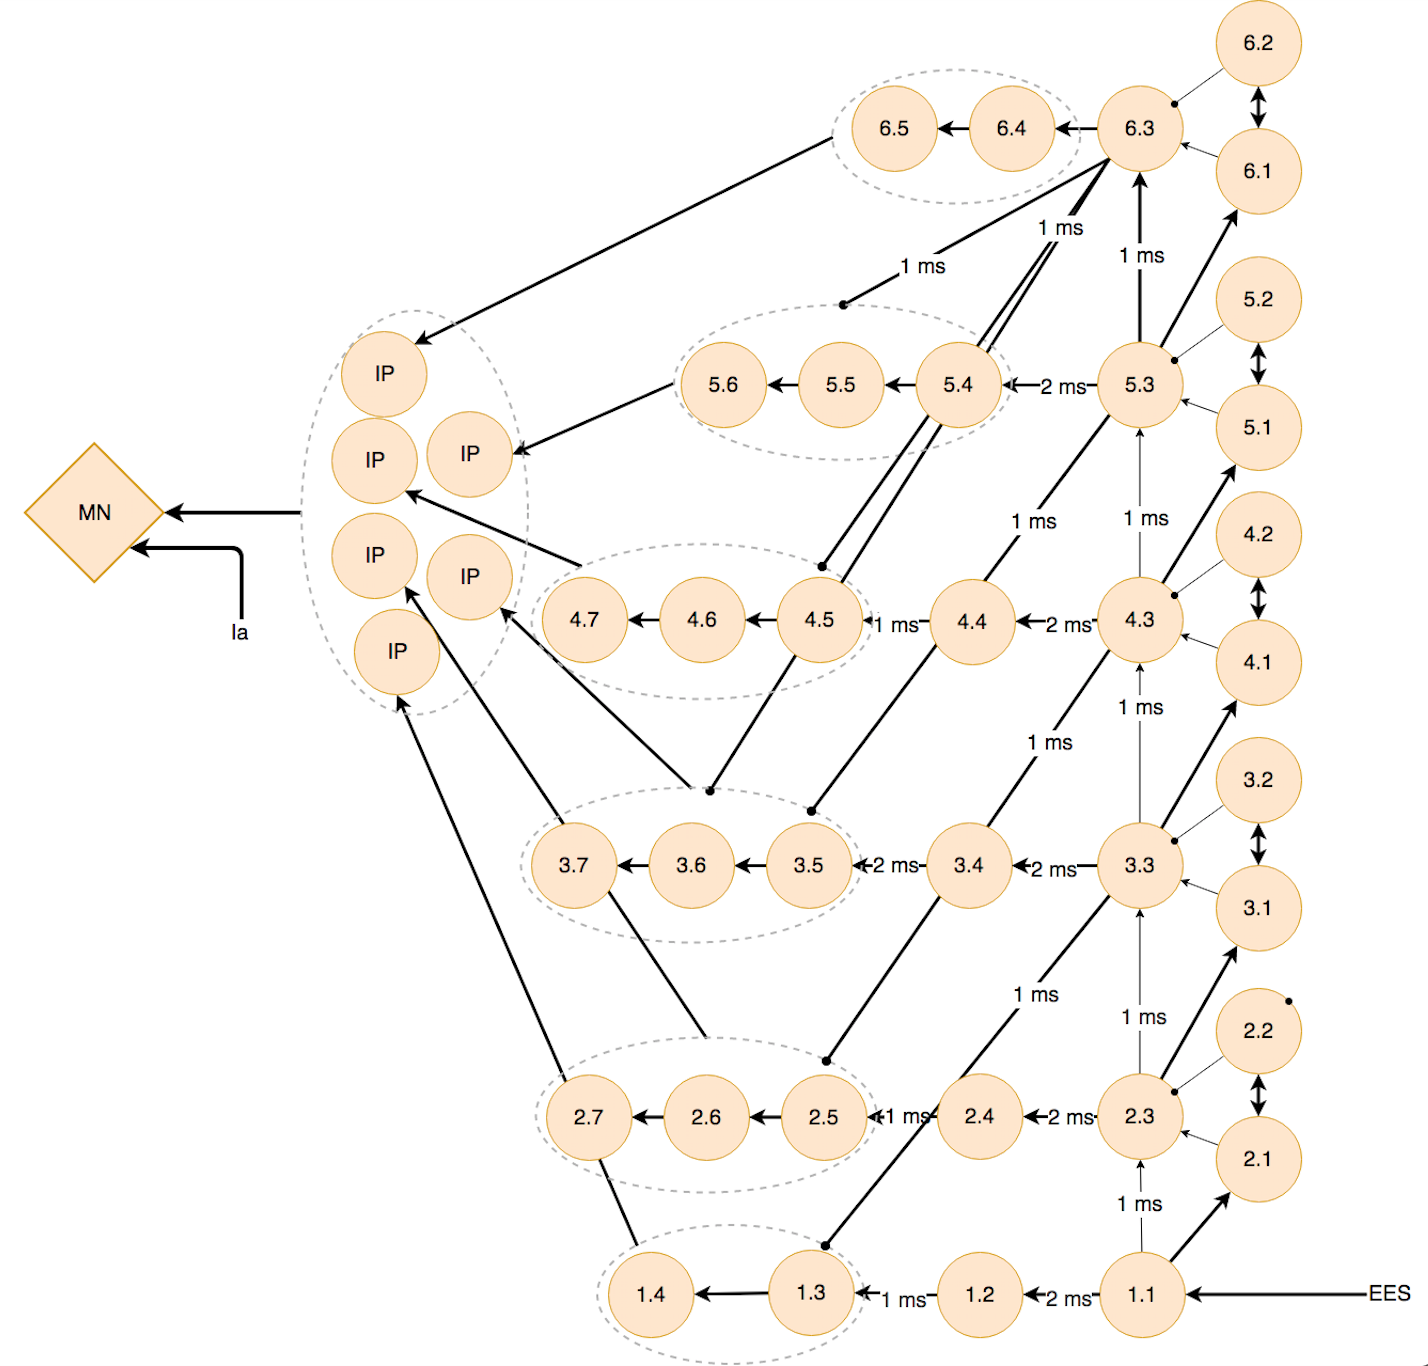
\includegraphics[width=1.0\textwidth]{new_cpg_concept_topology.png}
% \caption{\label{fig:cpg_topology}The proposed 6 layers topology of a mammalian CPG, where: 1.1-6.5 -- nuclei of the CPG, IP -- nuclei of the interneuronal pool, MN --motor neuron nucleus, EES the afferents projections with EES.}
% \end{figure}

\todo[inline]{add 10 iterations}

\subsection{Different percentages of inhibition (Neuron)}

We updated the value of weight of inhibitory connections. Half of the initial weight is an inhibition 50\%. One fifth of the initial weight is an inhibition 20\%. If there is no inhibition the weight is 0\%. Results are presented in Fig.\ref{fig:40_0}.

\begin{figure}[ht!]
	\centering
	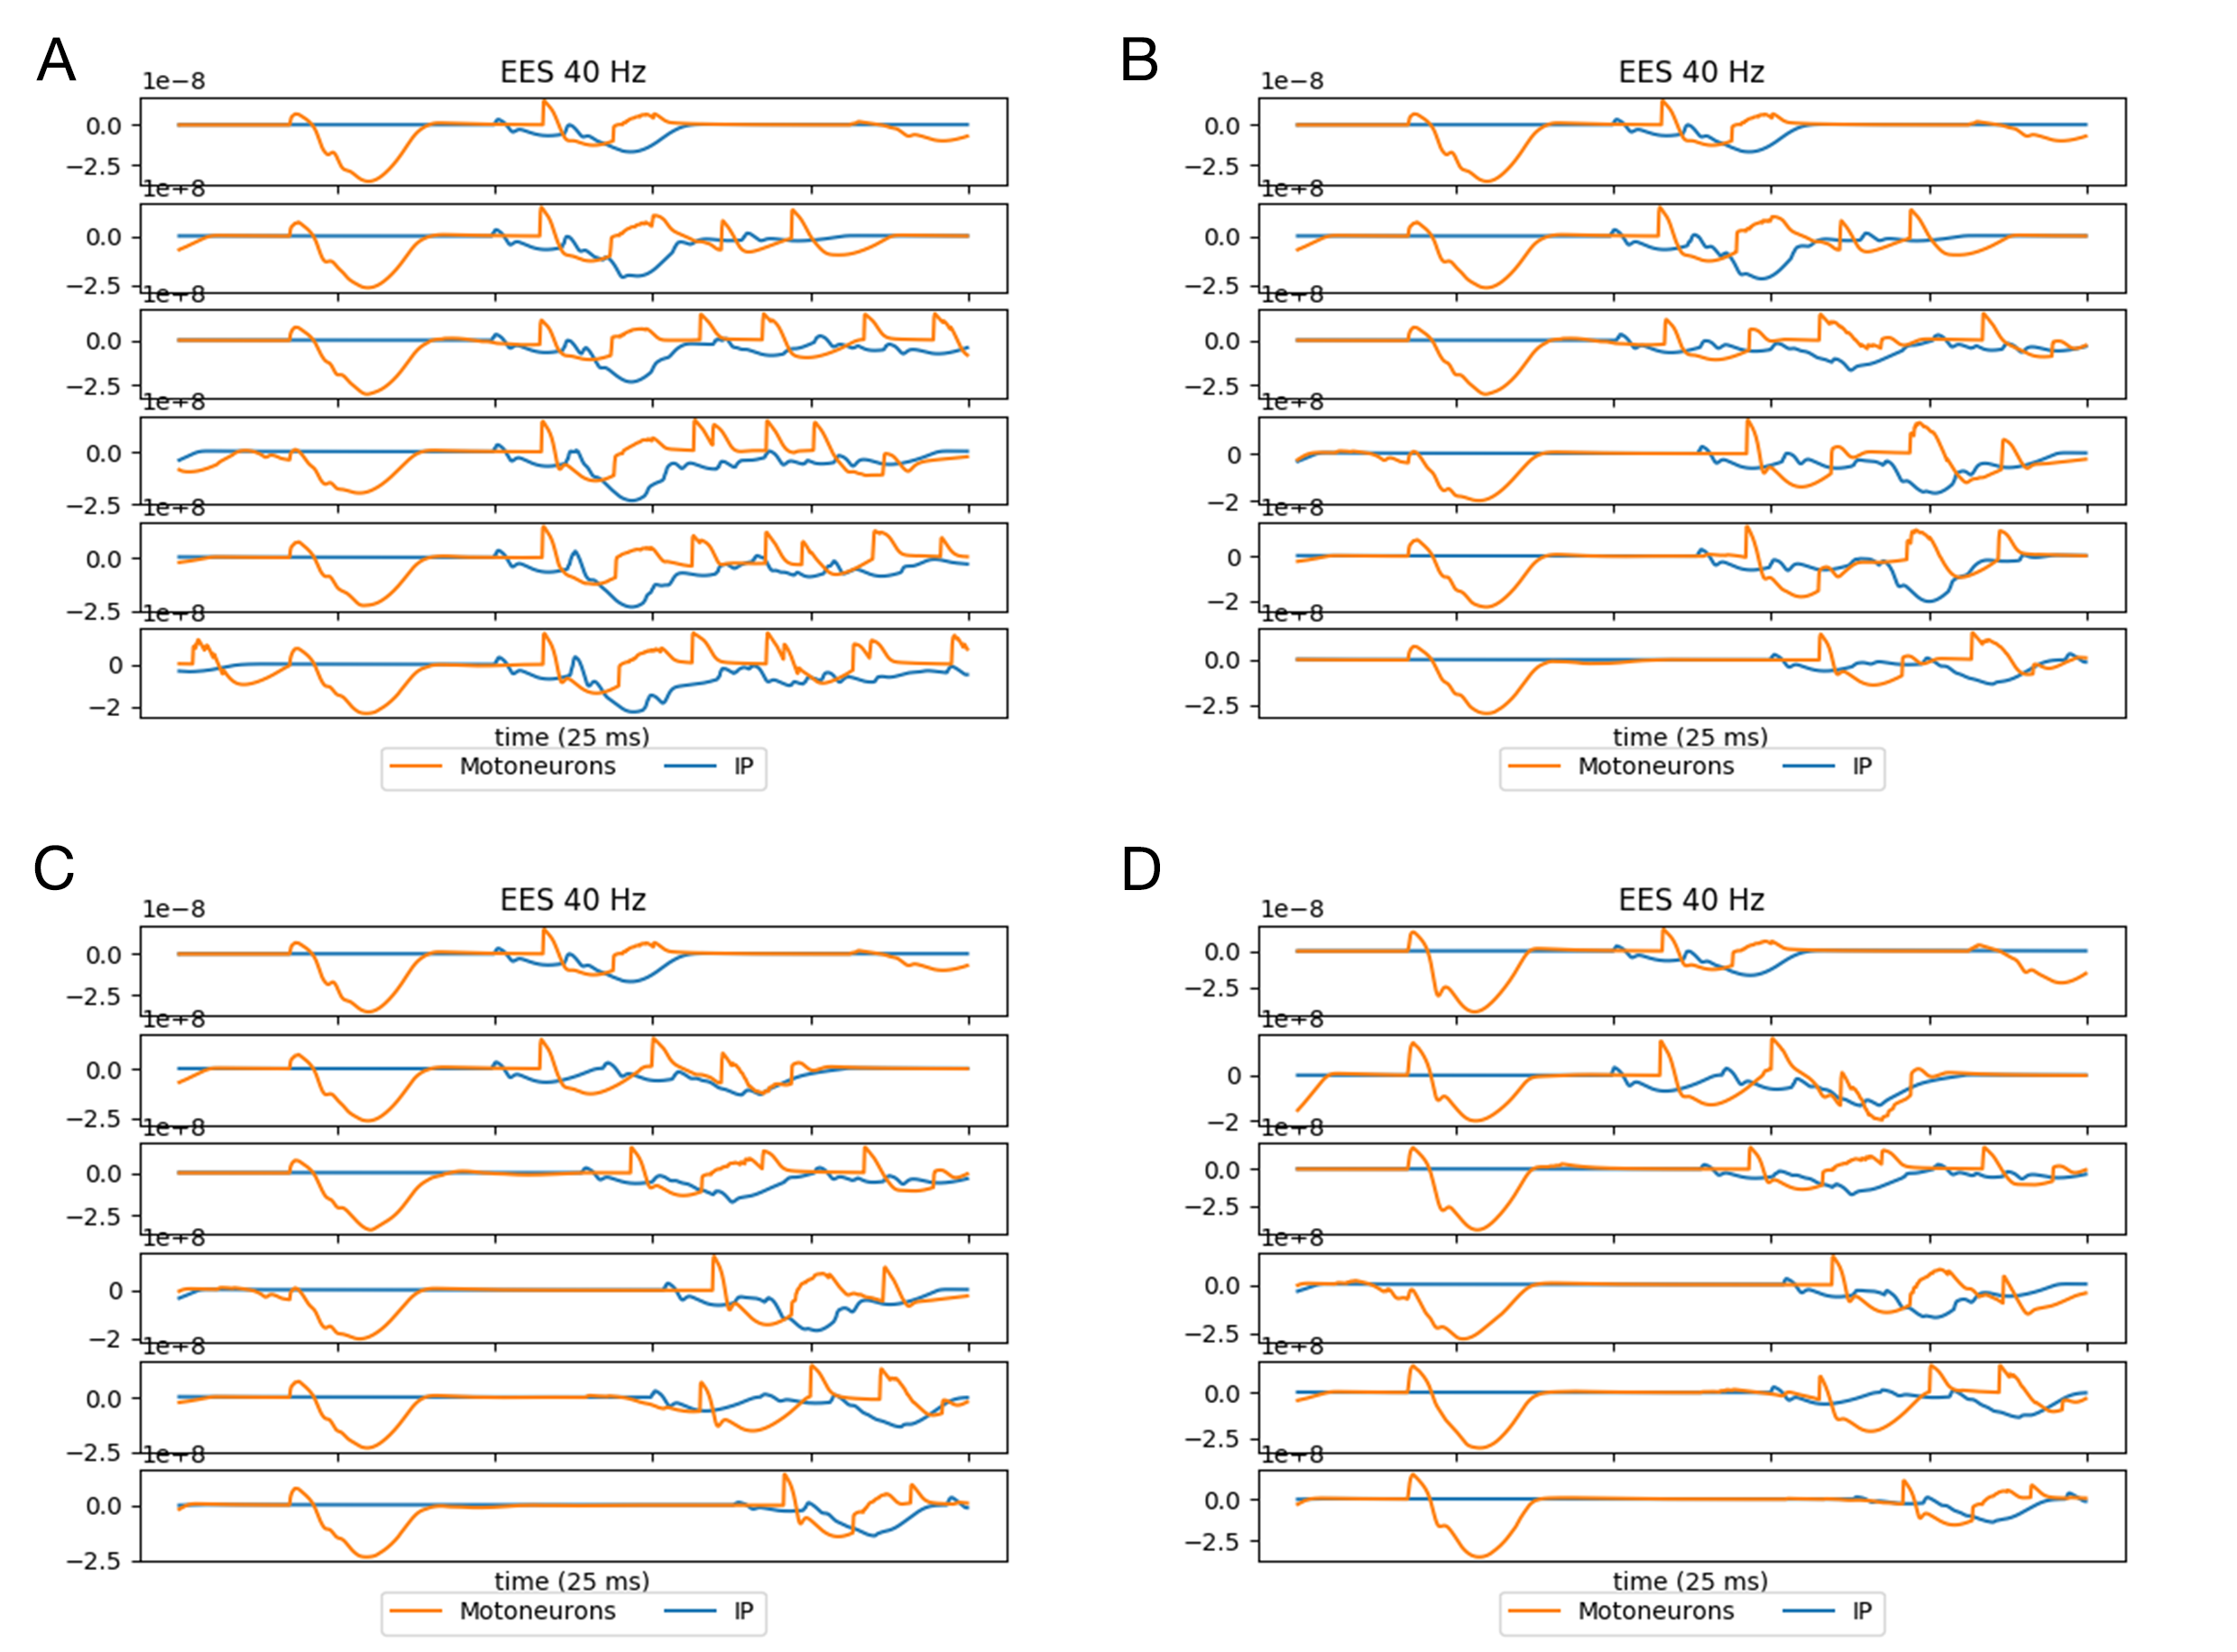
\includegraphics[width=1.0\textwidth]{results/diff_inh.png}
	\caption{The result of CPG simulation with 40 Hz of EES and different percentages of inhibition. The orange graph is motoneurons' extracellular potential. 
    A -- The spiking activity with the 40 Hz ESS and 0\% inhibition. 
    B -- The spiking activity with the 40 Hz ESS and 20\% inhibition. 
    C -- The spiking activity with the 40 Hz ESS and 50\% inhibition. 
    D -- The spiking activity with the 40 Hz ESS and 100\% inhibition.}
    \label{fig:40_0}
\end{figure}

\todo[inline]{Please add average data here.}

\subsection{Different inhibitory impact (NEST)}

We ran the simulation with different inhibitory coefficient from 0 to 1 and observed the same results while coefficient is over 0.25. It means 25\% of inhibition strength is a threshold value for our simulation, and we defined this value as an upper bound for the coefficient. A panel timescale is fixed and equals $25 ms$ for the all figures. Different layers response with an increasing delay. The delay between MR and LR on the myogram (Fig.\ref{fig:summary_inhibition_nest}) occurs due to inhibiting lower layers. For example: in the Fig.\ref{fig:summary_inhibition_nest}(A) the response on the third panel occurs later than on the second one due to the first layer was inhibited. By decreasing inhibitory strength we  expect layer will  be inhibited lesser and fire after every EES, we observe same delays between MR and LR in all panels. Moreover, if layers are not inhibited and fire after every pulse the result amplitude have to be higher than case of several layers are inhibited due to merging layers activity.

\begin{figure}[ht!]
	\centering
	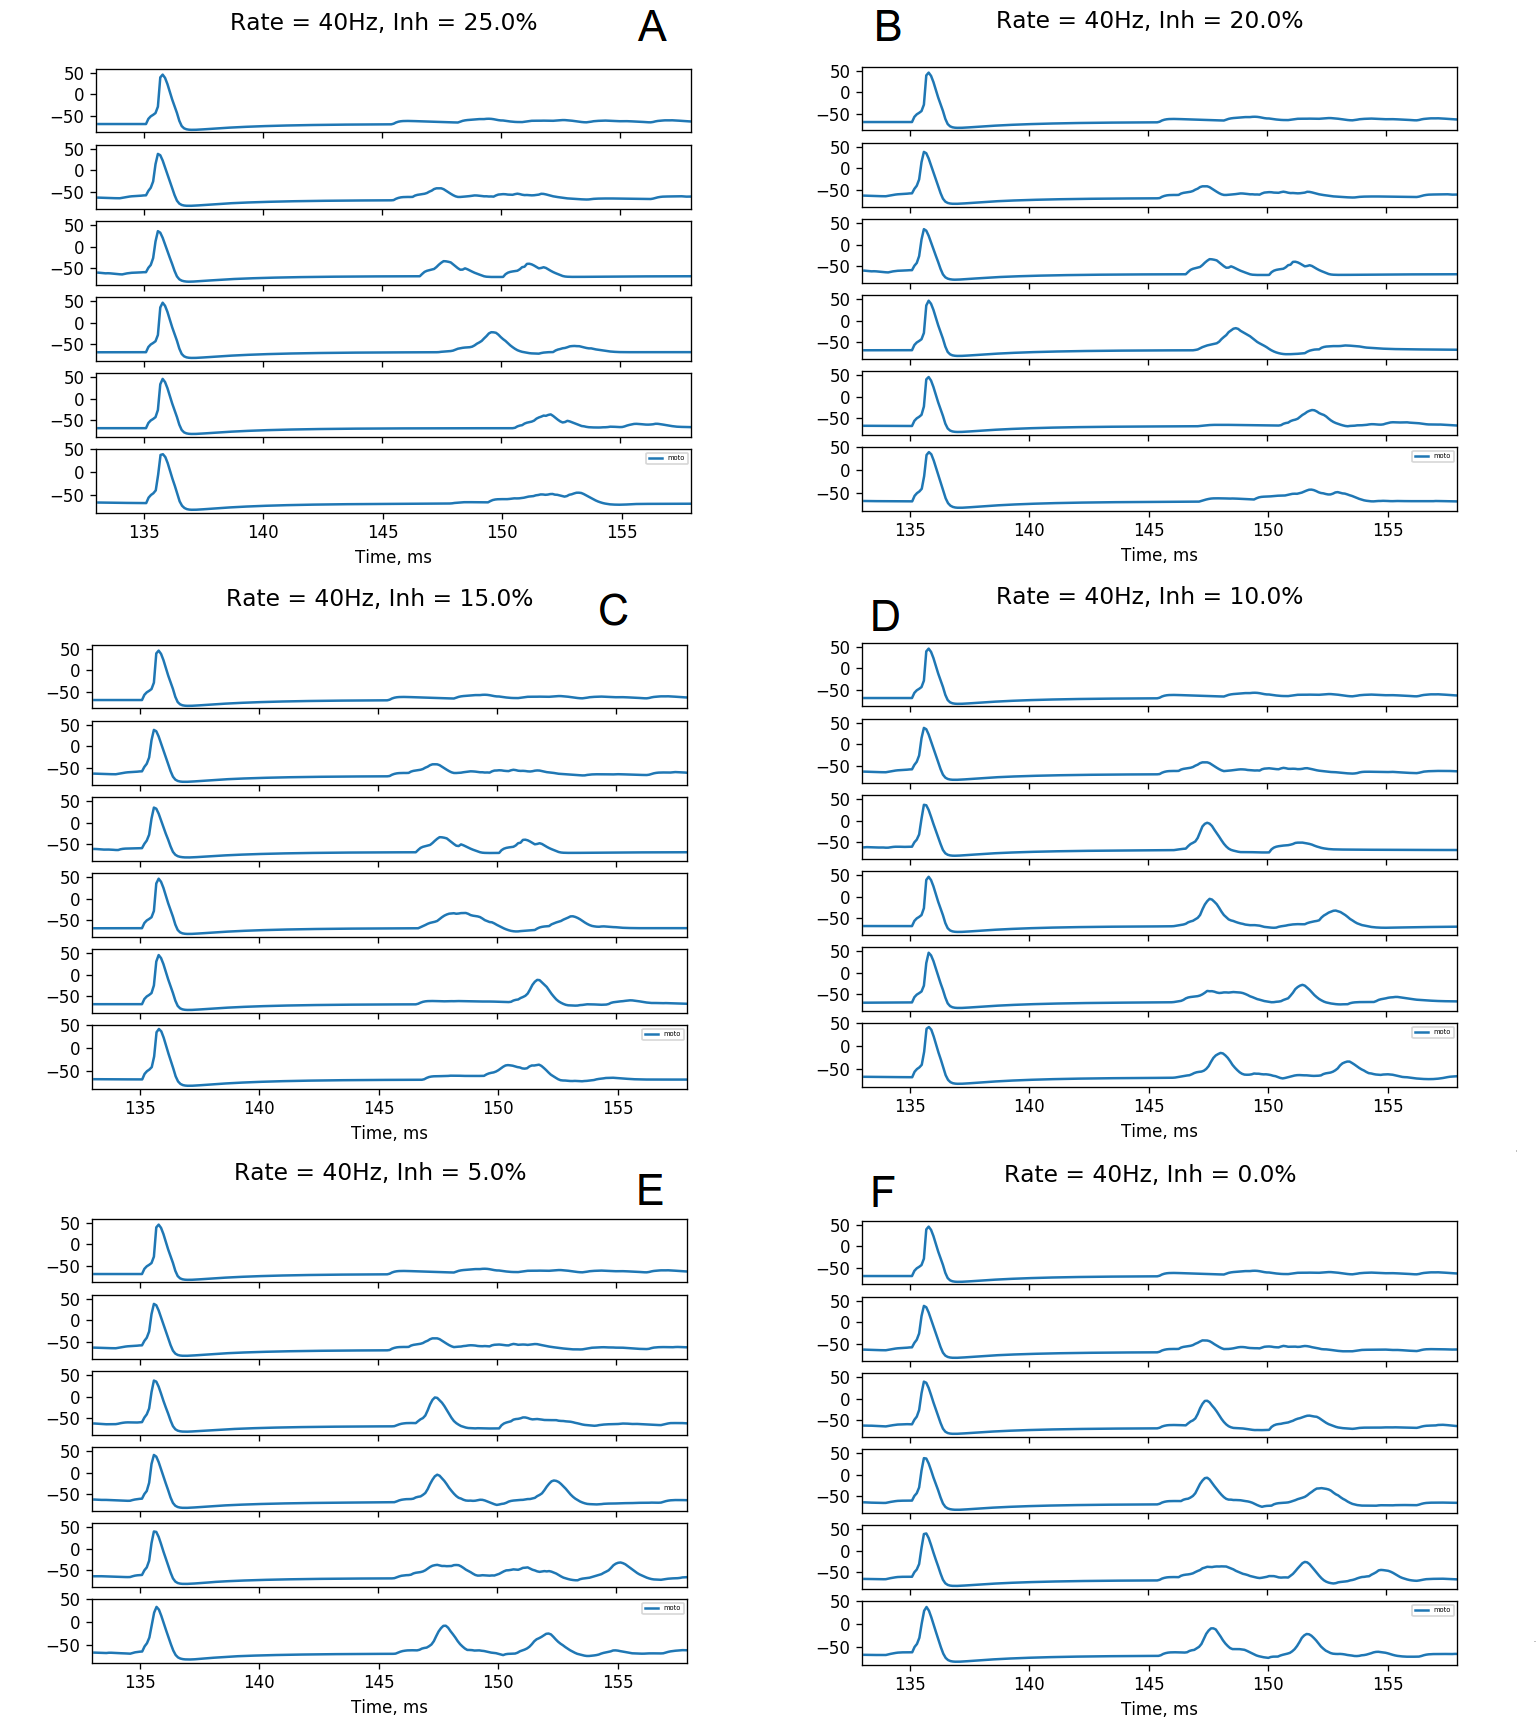
\includegraphics[width=1.0\textwidth]{results/summary_inhibition_nest.png}
	\caption{Results of the CPG simulation with 40 Hz of EES and 0--25\% of inhibition via NEST simulator. 
    \emph{A} -- 25\%, the base level of inhibition to reproduce the Fig.\ref{fig:myogram_origin}-like results 
    \emph{B} -- 20\%, 5-th and 6-th panels layers start firing with minimal delay but with lower amplitude in comparison to 25\% due to 1-st layer stays active. 
    \emph{C} -- 15\%, similar to 20\% but with higher amplitude due to less inhibition. 
    \emph{D} -- 10\%, minimal delays between MR and LR, with higher overall amplitude than 15\% due to the low inhibition. 
    \emph{E} -- 5\%, minimal delay and higher amplitude compared to 10\% inhibition. 
    \emph{F} -- 0\%, minimal delay, the highest amplitude due to no inhibition.}
    \label{fig:summary_inhibition_nest}
\end{figure}

\todo[inline]{We need to come with some comparison between results from Neuron and NEST}

\subsection{Different EES frequency (Neuron)}

We updated the value of interval of EES stimulation. The value is 50 ms for 20 Hz, 33 ms for 30 Hz, 20 ms for 50 Hz, 17 ms for 60 Hz. Results are presented in Fig.\ref{fig:30_100}.

\begin{figure}[ht!]
	\centering
	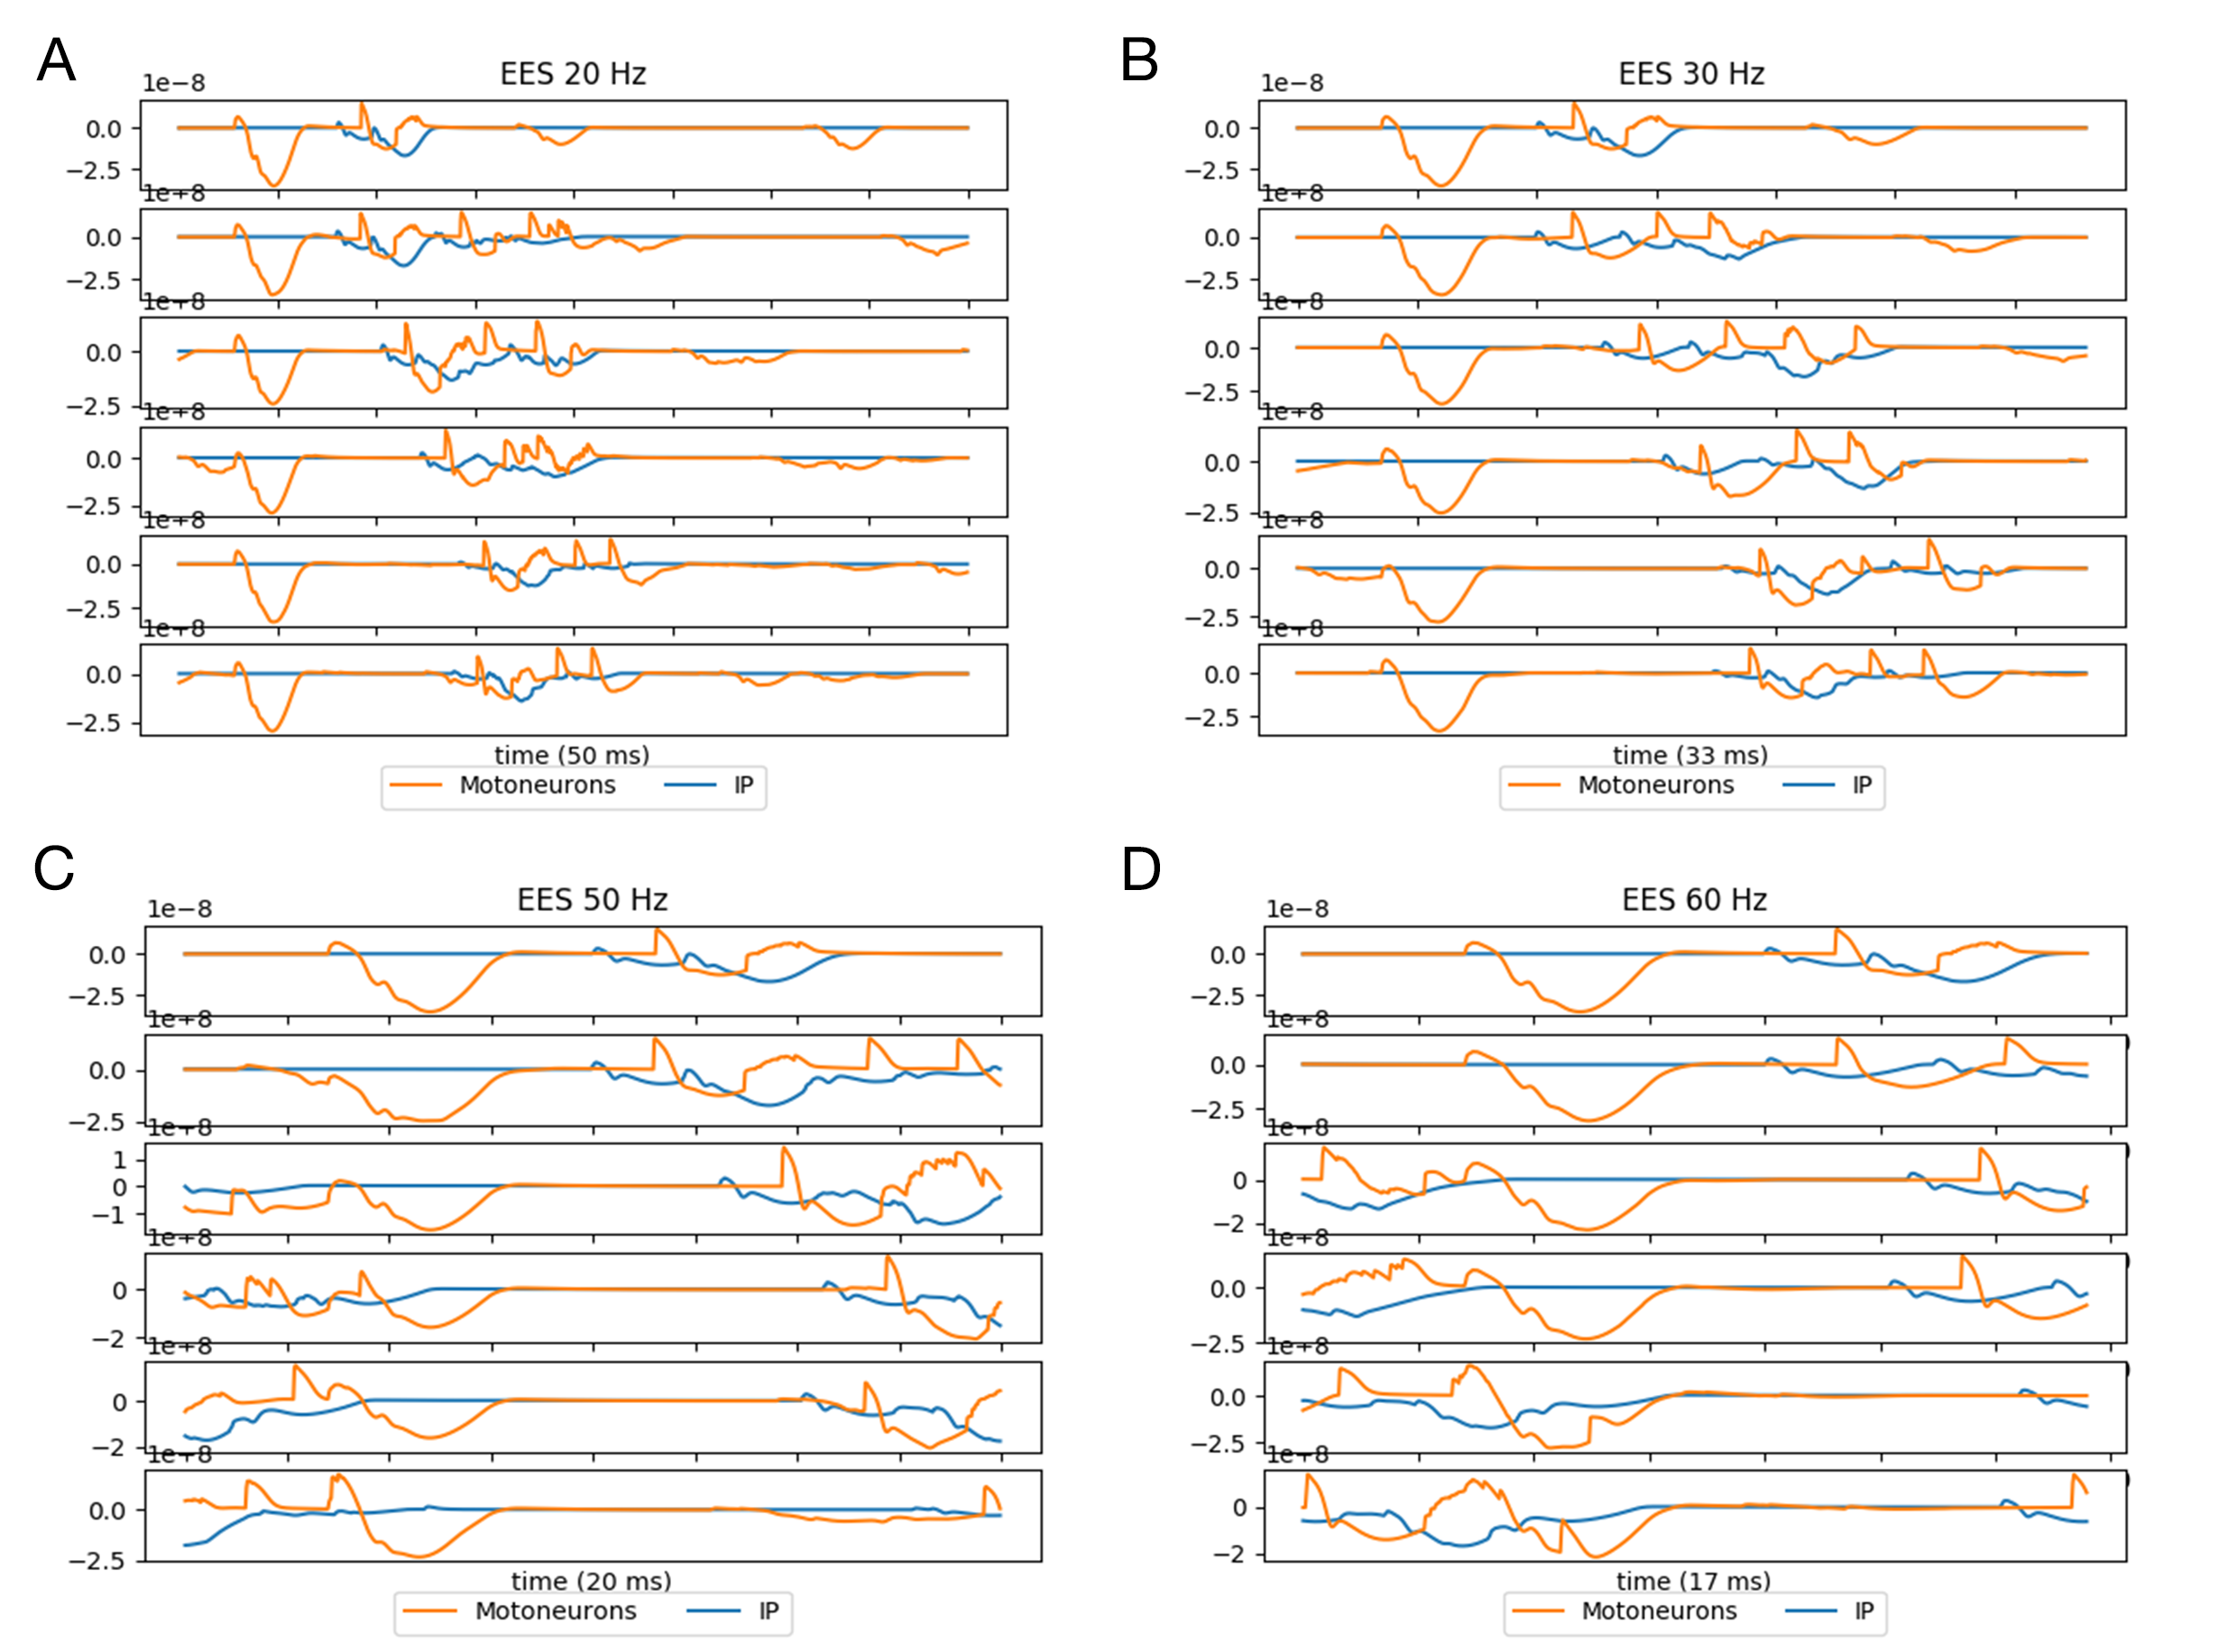
\includegraphics[width=1.0\textwidth]{results/diff_freq.png}
	\caption{The result of CPG simulation with different EES frequency and 100\% of inhibition. The orange graph is motoneurons' extracellular potential. 
    A -- The spiking activity with the 20 Hz ESS and 100\% inhibition. 
    B -- The spiking activity with the 30 Hz ESS and 100\% inhibition. 
    C -- The spiking activity with the 50 Hz ESS and 100\% inhibition. 
    D -- The spiking activity with the 60 Hz ESS and 100\% inhibition.}
    \label{fig:30_100}
\end{figure}

\todo[inline]{Need average}

\subsection{Different EES frequency (NEST)}

We run simulation with different stimulation rates from 20 Hz to 80 Hz. Panel timescale isn’t fixed and corresponds the period between MRs. For example, the period equals 25 ms for 40 Hz and 50 ms for 20 Hz. Results are presented in Fig.\ref{fig:nest_summary_rates}.

\begin{figure}[ht!]
	\centering
	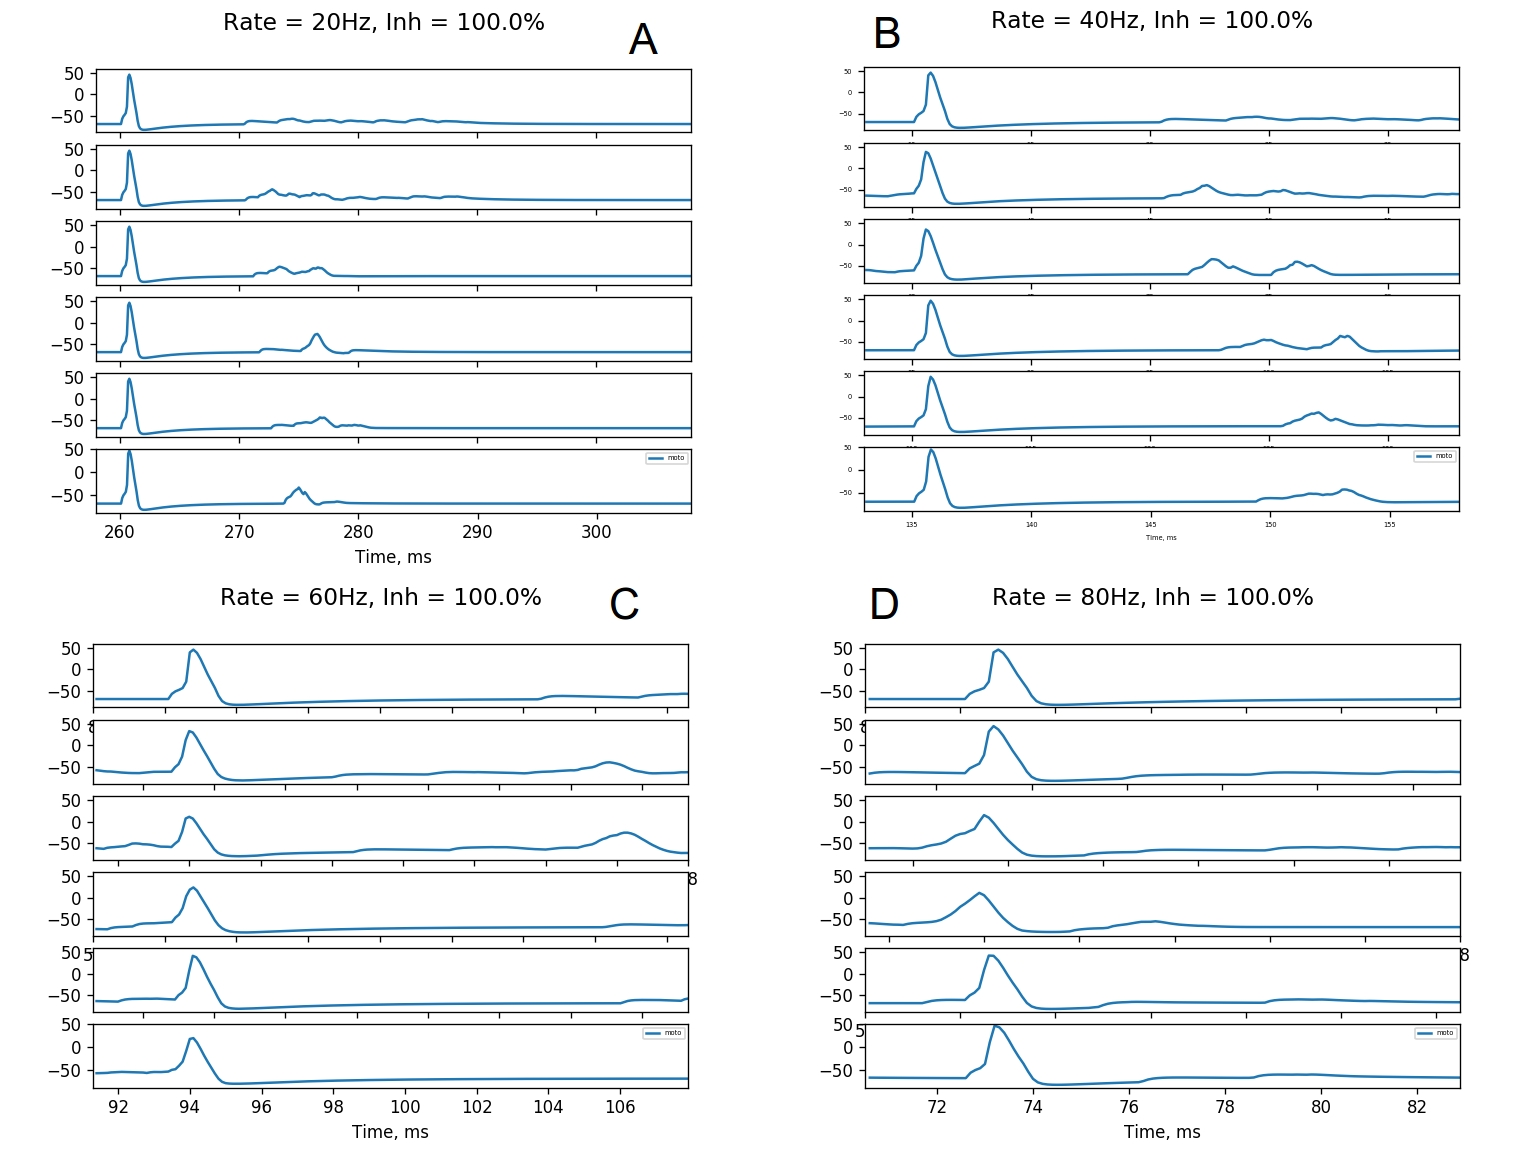
\includegraphics[width=1.0\textwidth]{results/summary_rates.jpg}
	\caption{The result of CPG simulation with different frequency of EES from 20 Hz to 80 Hz and 100\% of inhibition via NEST simulator. 
    \emph{A} -- 20 Hz, all LRs are short relatively to panel width. 
    \emph{B} -- 40 Hz. 
    \emph{C} -- 60 Hz, stimulation periods become shorter, many LRs fill several panels due to fixed response duration. 
    \emph{D} -- 80 Hz, panels too short, fixed responses fill all the space of panels.}
    \label{fig:nest_summary_rates}
\end{figure}

\begin{figure}[ht!]
	\centering
	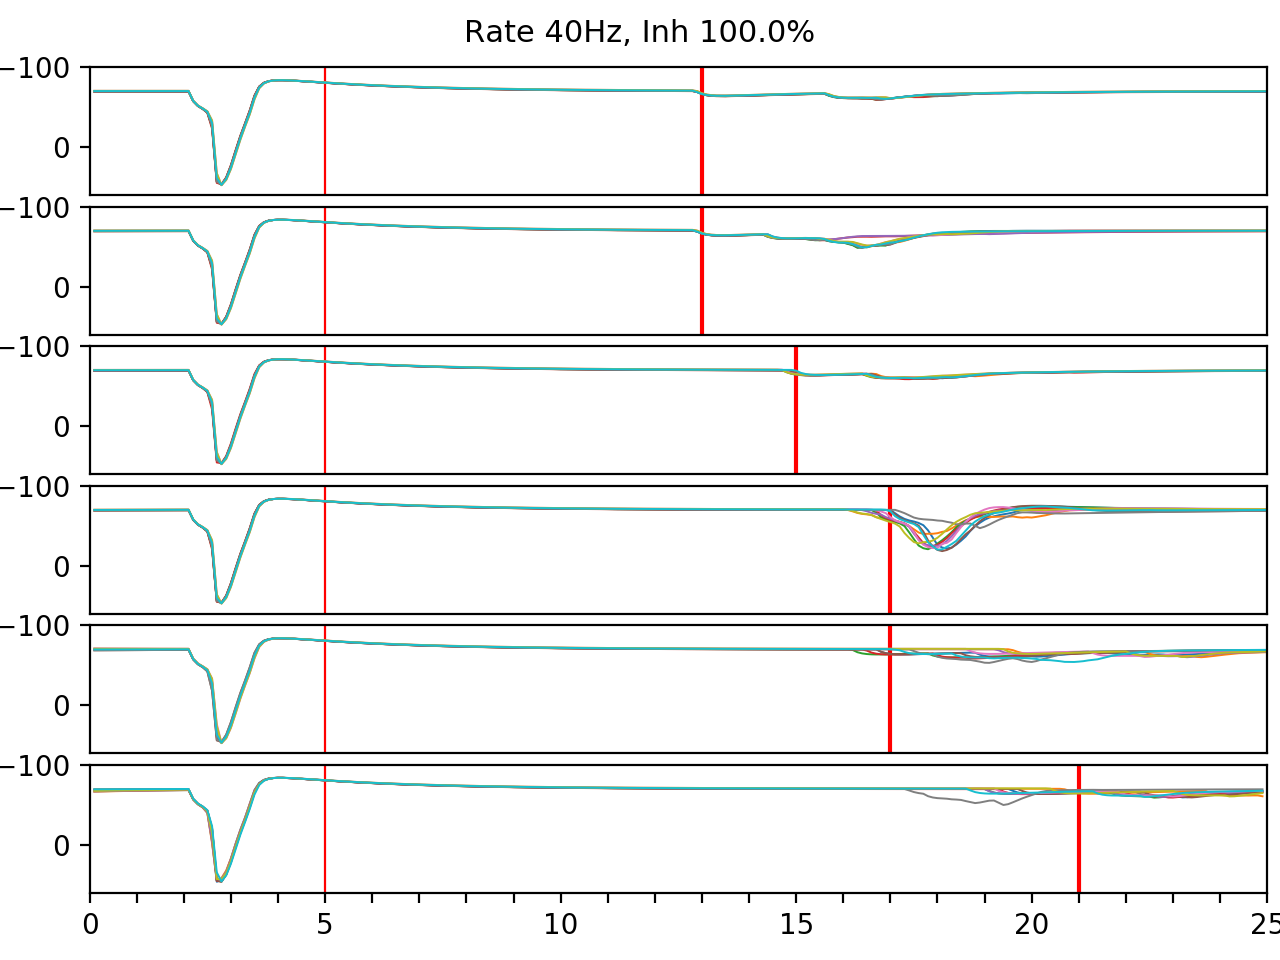
\includegraphics[width=0.5\textwidth]{results/slices40Hz-1_0Inh-6sublevels_mean.png}
	\caption{The result of the new topology.
    \todo[inline]{TODO: make the diagram in one style}
    }
    \label{fig:nest_new_results}
\end{figure}


\todo[inline]{Same, need comparison}


\todo[inline]{
LAVROV: Please see below a few samples of EMG activity under different conditions. We have to decide what data we can use for comparison with the model. 
Riaz could you please look what is available for analysis from our current results?}

\begin{figure}[ht!]
	\centering
	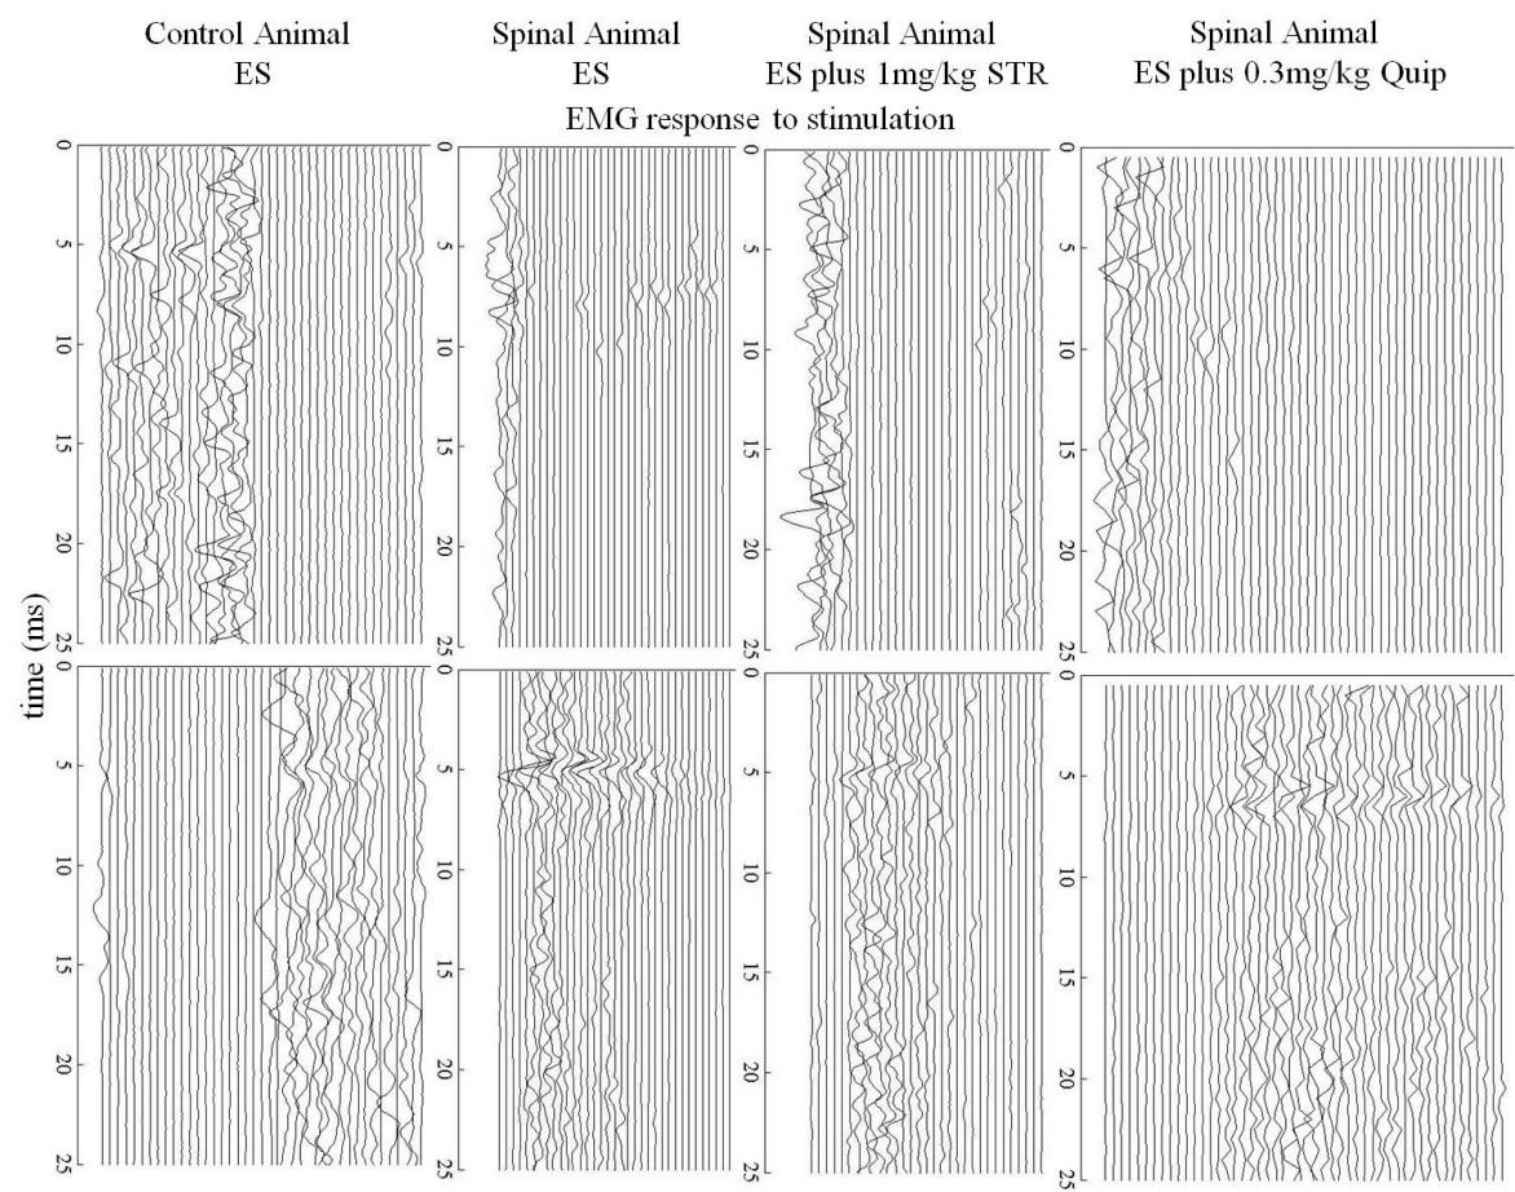
\includegraphics[width=1\textwidth]{new_pic/pic1.png}
	\caption{
    \todo[inline]{LAVROV: CNT vs. SCI vs. SCI+STR vs. SCI+5HT:}
    Modulation of the monosynaptic (MR) and polysynaptic (PC) responses under different conditions. We see a consistent MR and PC in the TA muscle response under the three spinal conditions, whereas there is a consistent MR in the ES case and the ES plus quipazine case but this is lost in the ES plus strychnine case. PC responses are seen in the first half of the burst in the ES case, but is seen throughout the burst in the ES plus strychnine and the ES plus quipazine cases. The intact animals, shows a double burst with activation throughout in the TA and a single burst with activation throughout in the soleus case. It is difficult to separate the MR and the PC in the intact case.
    }
    \label{fig:lavrov_updates1}
\end{figure}


\begin{figure}[ht!]
	\centering
	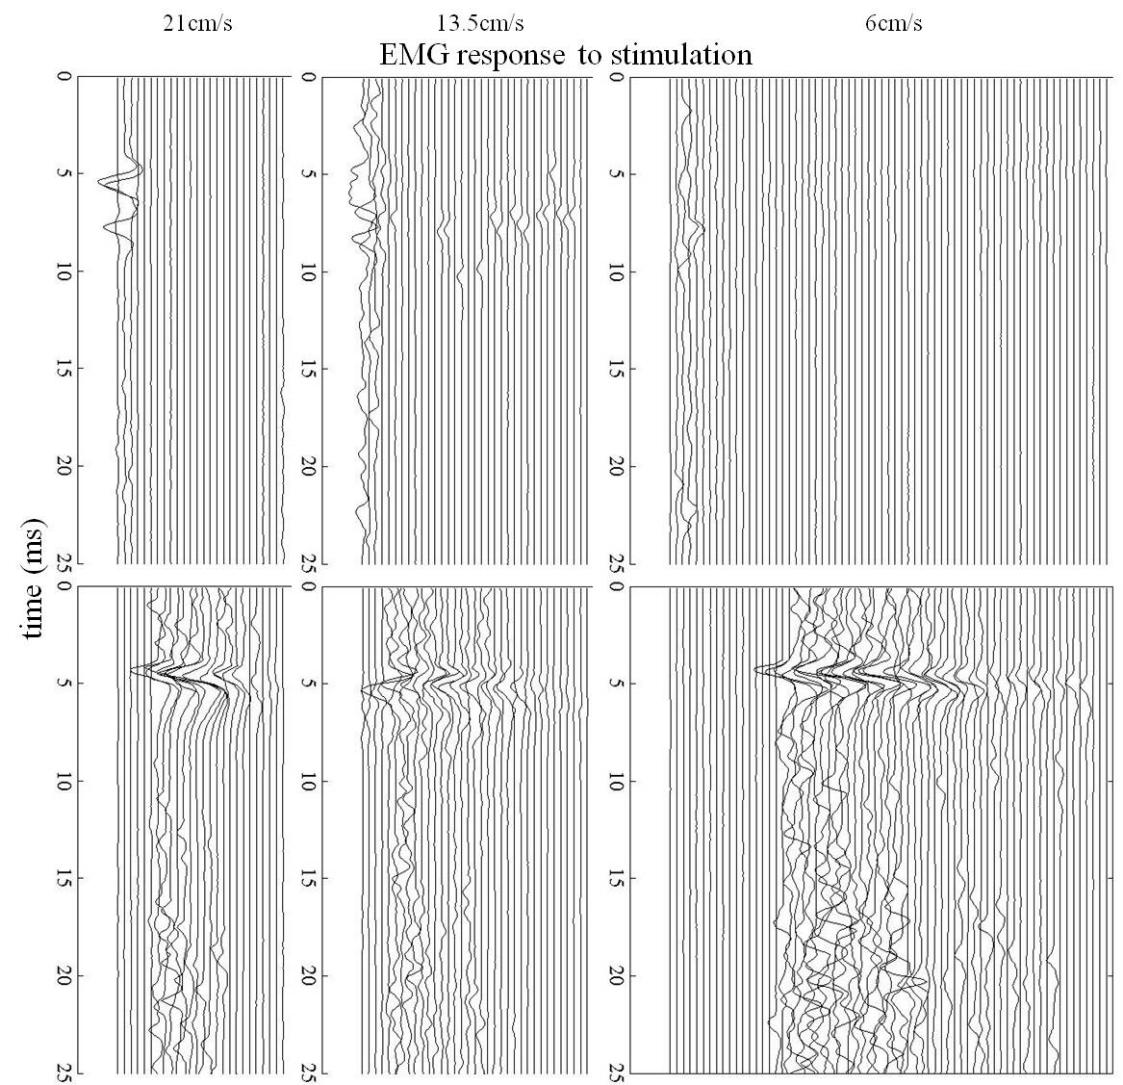
\includegraphics[width=1\textwidth]{new_pic/pic2.png}
	\caption{
    \todo[inline]{LAVROV: Speed}
    Modulation of monosynaptic and polysynaptic responses at different speeds of treadmill stepping in spinal rats.
    }
    \label{fig:lavrov_updates2}
\end{figure}

\begin{figure}[ht!]
	\centering
	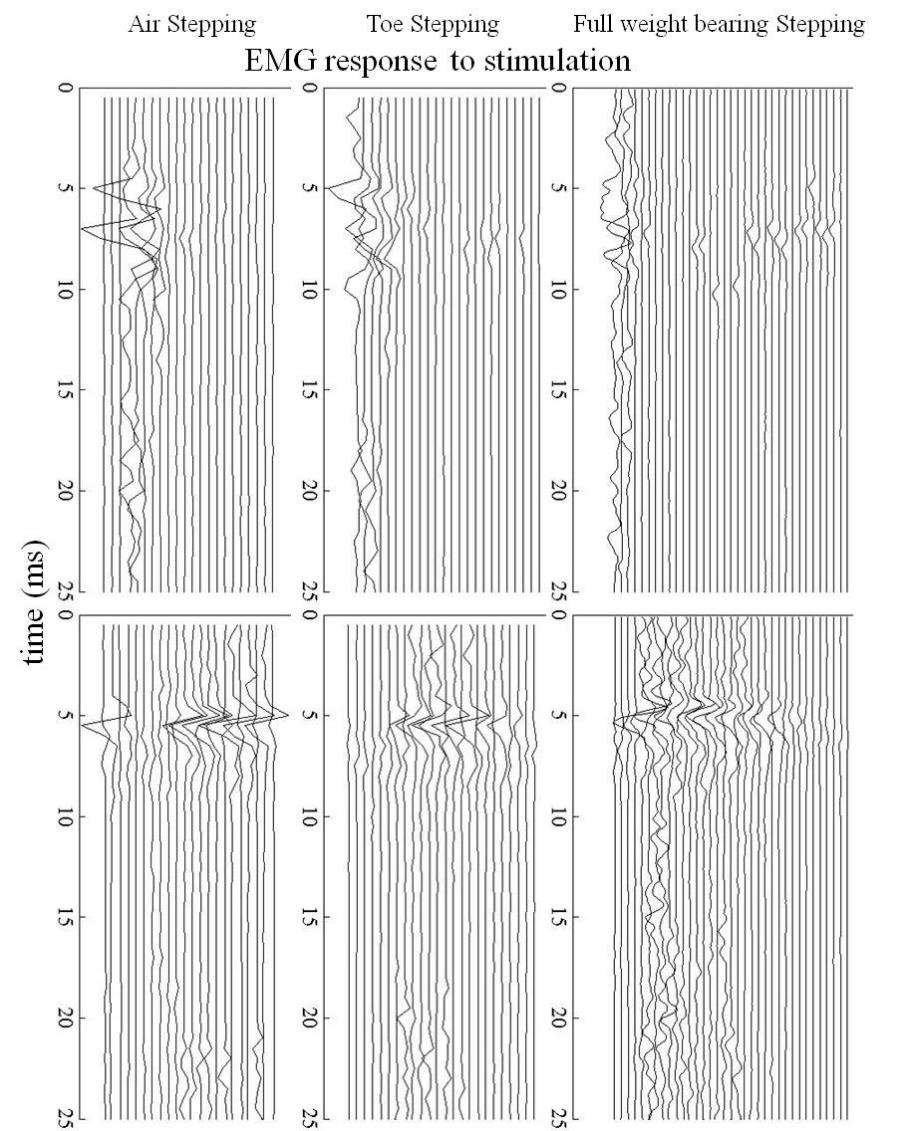
\includegraphics[width=1\textwidth]{new_pic/pic3.png}
	\caption{
    \todo[inline]{LAVROV: Body weight support:}
    Modulation of monosynaptic and polysynaptic responses under different body weight support conditions. A consistent MR and PC (throughout the burst) in the TA muscle response under the three conditions, whereas there is a consistent MR throughout the burst in the three cases. PC responses are seen in the first half of the burst in all the cases, but the number of PC responses are increasing as the amount of body weight support provided increases. 
    }
    \label{fig:lavrov_updates3}
\end{figure}

\begin{figure}[ht!]
	\centering
	\caption{
    \todo[inline]{LAVROV: Different frequencies of stimulation}
    }
    \label{fig:lavrov_updates4}
\end{figure}

\newpage

\bibliographystyle{apalike}
\bibliography{bib2018}

\end{document}
